\documentclass[twoside]{book}

% Packages required by doxygen
\usepackage{fixltx2e}
\usepackage{calc}
\usepackage{doxygen}
\usepackage[export]{adjustbox} % also loads graphicx
\usepackage{graphicx}
\usepackage[utf8]{inputenc}
\usepackage{makeidx}
\usepackage{multicol}
\usepackage{multirow}
\PassOptionsToPackage{warn}{textcomp}
\usepackage{textcomp}
\usepackage[nointegrals]{wasysym}
\usepackage[table]{xcolor}

% Font selection
\usepackage[T1]{fontenc}
\usepackage[scaled=.90]{helvet}
\usepackage{courier}
\usepackage{amssymb}
\usepackage{sectsty}
\renewcommand{\familydefault}{\sfdefault}
\allsectionsfont{%
  \fontseries{bc}\selectfont%
  \color{darkgray}%
}
\renewcommand{\DoxyLabelFont}{%
  \fontseries{bc}\selectfont%
  \color{darkgray}%
}
\newcommand{\+}{\discretionary{\mbox{\scriptsize$\hookleftarrow$}}{}{}}

% Page & text layout
\usepackage{geometry}
\geometry{%
  a4paper,%
  top=2.5cm,%
  bottom=2.5cm,%
  left=2.5cm,%
  right=2.5cm%
}
\tolerance=750
\hfuzz=15pt
\hbadness=750
\setlength{\emergencystretch}{15pt}
\setlength{\parindent}{0cm}
\setlength{\parskip}{3ex plus 2ex minus 2ex}
\makeatletter
\renewcommand{\paragraph}{%
  \@startsection{paragraph}{4}{0ex}{-1.0ex}{1.0ex}{%
    \normalfont\normalsize\bfseries\SS@parafont%
  }%
}
\renewcommand{\subparagraph}{%
  \@startsection{subparagraph}{5}{0ex}{-1.0ex}{1.0ex}{%
    \normalfont\normalsize\bfseries\SS@subparafont%
  }%
}
\makeatother

% Headers & footers
\usepackage{fancyhdr}
\pagestyle{fancyplain}
\fancyhead[LE]{\fancyplain{}{\bfseries\thepage}}
\fancyhead[CE]{\fancyplain{}{}}
\fancyhead[RE]{\fancyplain{}{\bfseries\leftmark}}
\fancyhead[LO]{\fancyplain{}{\bfseries\rightmark}}
\fancyhead[CO]{\fancyplain{}{}}
\fancyhead[RO]{\fancyplain{}{\bfseries\thepage}}
\fancyfoot[LE]{\fancyplain{}{}}
\fancyfoot[CE]{\fancyplain{}{}}
\fancyfoot[RE]{\fancyplain{}{\bfseries\scriptsize Generated by Doxygen }}
\fancyfoot[LO]{\fancyplain{}{\bfseries\scriptsize Generated by Doxygen }}
\fancyfoot[CO]{\fancyplain{}{}}
\fancyfoot[RO]{\fancyplain{}{}}
\renewcommand{\footrulewidth}{0.4pt}
\renewcommand{\chaptermark}[1]{%
  \markboth{#1}{}%
}
\renewcommand{\sectionmark}[1]{%
  \markright{\thesection\ #1}%
}

% Indices & bibliography
\usepackage{natbib}
\usepackage[titles]{tocloft}
\setcounter{tocdepth}{3}
\setcounter{secnumdepth}{5}
\makeindex

% Hyperlinks (required, but should be loaded last)
\usepackage{ifpdf}
\ifpdf
  \usepackage[pdftex,pagebackref=true]{hyperref}
\else
  \usepackage[ps2pdf,pagebackref=true]{hyperref}
\fi
\hypersetup{%
  colorlinks=true,%
  linkcolor=blue,%
  citecolor=blue,%
  unicode%
}

% Custom commands
\newcommand{\clearemptydoublepage}{%
  \newpage{\pagestyle{empty}\cleardoublepage}%
}

\usepackage{caption}
\captionsetup{labelsep=space,justification=centering,font={bf},singlelinecheck=off,skip=4pt,position=top}

%===== C O N T E N T S =====

\begin{document}

% Titlepage & ToC
\hypersetup{pageanchor=false,
             bookmarksnumbered=true,
             pdfencoding=unicode
            }
\pagenumbering{alph}
\begin{titlepage}
\vspace*{7cm}
\begin{center}%
{\Large doxygen L\+AY T\+E\+R\+T\+R\+A\+IS }\\
\vspace*{1cm}
{\large Generated by Doxygen 1.8.13}\\
\end{center}
\end{titlepage}
\clearemptydoublepage
\pagenumbering{roman}
\tableofcontents
\clearemptydoublepage
\pagenumbering{arabic}
\hypersetup{pageanchor=true}

%--- Begin generated contents ---
\chapter{Hierarchical Index}
\section{Class Hierarchy}
This inheritance list is sorted roughly, but not completely, alphabetically\+:\begin{DoxyCompactList}
\item \contentsline{section}{Couple}{\pageref{class_couple}}{}
\item \contentsline{section}{Notes\+Manager2\+:\+:Handler}{\pageref{struct_notes_manager2_1_1_handler}}{}
\item \contentsline{section}{Manager$<$ T $>$}{\pageref{class_manager}}{}
\item \contentsline{section}{Manager$<$ note $>$}{\pageref{class_manager}}{}
\begin{DoxyCompactList}
\item \contentsline{section}{Notes\+Manager2}{\pageref{class_notes_manager2}}{}
\end{DoxyCompactList}
\item \contentsline{section}{Manager$<$ Relation $>$}{\pageref{class_manager}}{}
\begin{DoxyCompactList}
\item \contentsline{section}{Relation\+Manager}{\pageref{class_relation_manager}}{}
\end{DoxyCompactList}
\item \contentsline{section}{note}{\pageref{classnote}}{}
\begin{DoxyCompactList}
\item \contentsline{section}{article}{\pageref{classarticle}}{}
\item \contentsline{section}{media}{\pageref{classmedia}}{}
\item \contentsline{section}{tache}{\pageref{classtache}}{}
\end{DoxyCompactList}
\item \contentsline{section}{Notes\+Exception}{\pageref{class_notes_exception}}{}
\item Q\+Main\+Window\begin{DoxyCompactList}
\item \contentsline{section}{Fen\+Principale}{\pageref{class_fen_principale}}{}
\end{DoxyCompactList}
\item Q\+Widget\begin{DoxyCompactList}
\item \contentsline{section}{fenetre\+\_\+anciennes\+\_\+versions}{\pageref{classfenetre__anciennes__versions}}{}
\item \contentsline{section}{fenetre\+\_\+creation\+\_\+note}{\pageref{classfenetre__creation__note}}{}
\item \contentsline{section}{fenetre\+\_\+creation\+\_\+relation}{\pageref{classfenetre__creation__relation}}{}
\end{DoxyCompactList}
\item \contentsline{section}{Relation}{\pageref{class_relation}}{}
\end{DoxyCompactList}

\chapter{Class Index}
\section{Class List}
Here are the classes, structs, unions and interfaces with brief descriptions\+:\begin{DoxyCompactList}
\item\contentsline{section}{\hyperlink{classarticle}{article} \\*Classe fille de note }{\pageref{classarticle}}{}
\item\contentsline{section}{\hyperlink{class_couple}{Couple} }{\pageref{class_couple}}{}
\item\contentsline{section}{\hyperlink{classfenetre__anciennes__versions}{fenetre\+\_\+anciennes\+\_\+versions} }{\pageref{classfenetre__anciennes__versions}}{}
\item\contentsline{section}{\hyperlink{classfenetre__creation__note}{fenetre\+\_\+creation\+\_\+note} }{\pageref{classfenetre__creation__note}}{}
\item\contentsline{section}{\hyperlink{classfenetre__creation__relation}{fenetre\+\_\+creation\+\_\+relation} }{\pageref{classfenetre__creation__relation}}{}
\item\contentsline{section}{\hyperlink{class_fen_principale}{Fen\+Principale} }{\pageref{class_fen_principale}}{}
\item\contentsline{section}{\hyperlink{class_manager}{Manager$<$ T $>$} \\*Classe mère Template abstraite Managers }{\pageref{class_manager}}{}
\item\contentsline{section}{\hyperlink{classmedia}{media} \\*Classe fille de note }{\pageref{classmedia}}{}
\item\contentsline{section}{\hyperlink{classnote}{note} \\*Classe mère abstraite des types de notes }{\pageref{classnote}}{}
\item\contentsline{section}{\hyperlink{class_notes_exception}{Notes\+Exception} \\*Cette classe récupère un string correspondant à une erreur et a pour fonction de l\textquotesingle{}afficher sur la sortie standard }{\pageref{class_notes_exception}}{}
\item\contentsline{section}{\hyperlink{class_notes_manager2}{Notes\+Manager2} \\*Classe fille héritant de \hyperlink{class_manager}{Manager$<$note$>$} et chargée des notes. dispose du Deseign Pattern Singleton }{\pageref{class_notes_manager2}}{}
\item\contentsline{section}{\hyperlink{class_relation}{Relation} }{\pageref{class_relation}}{}
\item\contentsline{section}{\hyperlink{class_relation_manager}{Relation\+Manager} \\*Classe fille héritant de \hyperlink{class_manager}{Manager$<$\+Relation$>$} et chargée des relations. dispose du Deseign Pattern Singleton }{\pageref{class_relation_manager}}{}
\item\contentsline{section}{\hyperlink{classtache}{tache} \\*Classe fille de note }{\pageref{classtache}}{}
\end{DoxyCompactList}

\chapter{Class Documentation}
\hypertarget{classarticle}{}\section{article Class Reference}
\label{classarticle}\index{article@{article}}


Classe fille de note.  




{\ttfamily \#include $<$notes.\+h$>$}

Inheritance diagram for article\+:\begin{figure}[H]
\begin{center}
\leavevmode
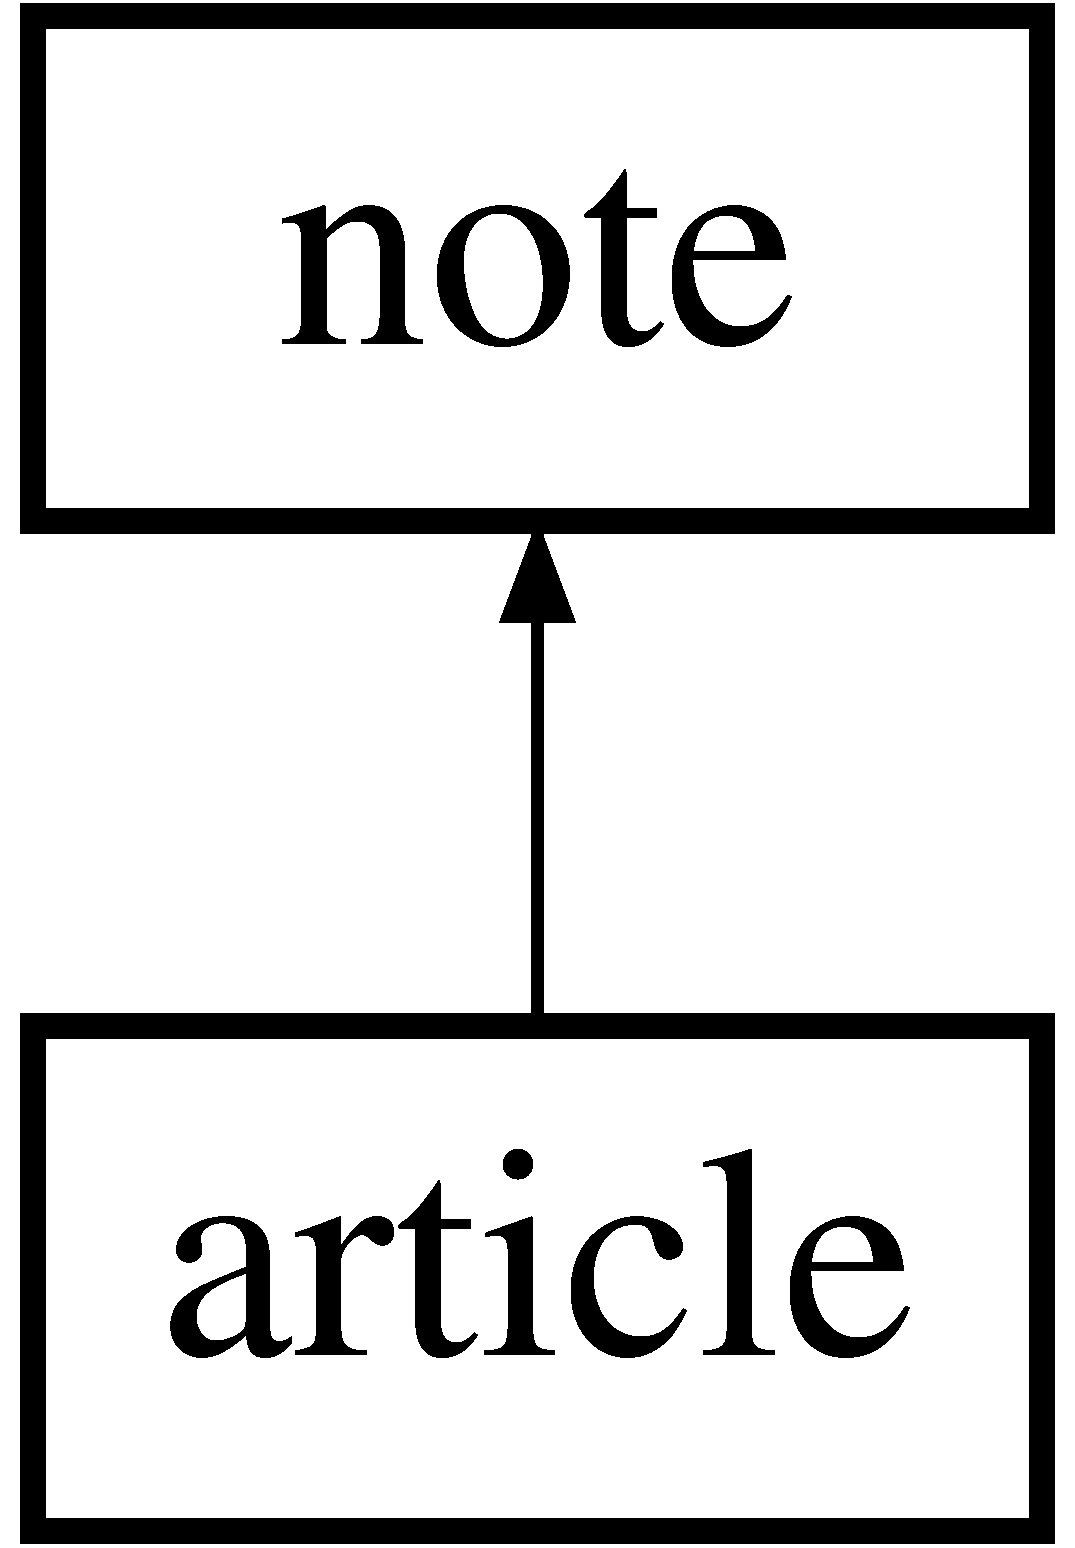
\includegraphics[height=2.000000cm]{classarticle}
\end{center}
\end{figure}
\subsection*{Public Member Functions}
\begin{DoxyCompactItemize}
\item 
\hyperlink{classarticle_a867baf47c29d2fb267ed4670d082d9c4}{article} (std\+::string i, std\+::string t, std\+::string txt, std\+::string crea=\char`\"{}\char`\"{}, std\+::string modif=\char`\"{}\char`\"{})
\begin{DoxyCompactList}\small\item\em constructeur similaire à celui de note. \end{DoxyCompactList}\item 
\mbox{\Hypertarget{classarticle_a126aafdac25309fab3eebf52e78e2083}\label{classarticle_a126aafdac25309fab3eebf52e78e2083}} 
\hyperlink{classarticle_a126aafdac25309fab3eebf52e78e2083}{article} (const \hyperlink{classarticle}{article} \&article\+\_\+a\+\_\+copier)
\begin{DoxyCompactList}\small\item\em constructeur de recopie de article. \end{DoxyCompactList}\item 
\mbox{\Hypertarget{classarticle_aedb5047877f01a317e1345f898f71bf3}\label{classarticle_aedb5047877f01a317e1345f898f71bf3}} 
virtual void \hyperlink{classarticle_aedb5047877f01a317e1345f898f71bf3}{afficher} (std\+::ostream \&f=std\+::cout) const
\begin{DoxyCompactList}\small\item\em appelle la fonction \hyperlink{classarticle_aedb5047877f01a317e1345f898f71bf3}{afficher()} de note (pas d\textquotesingle{}attribut supplémentaire). \end{DoxyCompactList}\end{DoxyCompactItemize}
\subsection*{Additional Inherited Members}


\subsection{Detailed Description}
Classe fille de note. 

cette classe n\textquotesingle{}ajoute pas de nouvel attribut car texte est commun à toutes les notes 

\subsection{Constructor \& Destructor Documentation}
\mbox{\Hypertarget{classarticle_a867baf47c29d2fb267ed4670d082d9c4}\label{classarticle_a867baf47c29d2fb267ed4670d082d9c4}} 
\index{article@{article}!article@{article}}
\index{article@{article}!article@{article}}
\subsubsection{\texorpdfstring{article()}{article()}}
{\footnotesize\ttfamily article\+::article (\begin{DoxyParamCaption}\item[{std\+::string}]{i,  }\item[{std\+::string}]{t,  }\item[{std\+::string}]{txt,  }\item[{std\+::string}]{crea = {\ttfamily \char`\"{}\char`\"{}},  }\item[{std\+::string}]{modif = {\ttfamily \char`\"{}\char`\"{}} }\end{DoxyParamCaption})\hspace{0.3cm}{\ttfamily [inline]}}



constructeur similaire à celui de note. 


\begin{DoxyParams}{Parameters}
{\em i} & \+: id unique de l\textquotesingle{}article \\
\hline
{\em t} & \+: titre de l\textquotesingle{}article \\
\hline
{\em txt} & \+: texte décrivant l\textquotesingle{}article \\
\hline
{\em crea} & \+: date de création de l\textquotesingle{}article \\
\hline
{\em modif} & \+: date de derniere modification de l\textquotesingle{}article \\
\hline
\end{DoxyParams}


The documentation for this class was generated from the following files\+:\begin{DoxyCompactItemize}
\item 
notes.\+h\item 
notes.\+cpp\end{DoxyCompactItemize}

\hypertarget{class_couple}{}\section{Couple Class Reference}
\label{class_couple}\index{Couple@{Couple}}


Classe définissant les couples.  




{\ttfamily \#include $<$relations.\+h$>$}

\subsection*{Public Member Functions}
\begin{DoxyCompactItemize}
\item 
\hyperlink{class_couple_aa1f1400e92e062c0ecdd6f81fdc47d07}{Couple} (\hyperlink{classnote}{note} \&note1, \hyperlink{classnote}{note} \&note2, std\+::string lab, bool ori)
\begin{DoxyCompactList}\small\item\em Constructeur de couple. \end{DoxyCompactList}\item 
\mbox{\Hypertarget{class_couple_a25c14d126cb78805740000253b32f6d7}\label{class_couple_a25c14d126cb78805740000253b32f6d7}} 
const \hyperlink{classnote}{note} \& \hyperlink{class_couple_a25c14d126cb78805740000253b32f6d7}{get\+Premiere} () const
\begin{DoxyCompactList}\small\item\em accesseur en lecture retournant une référence sur la première note du couple. \end{DoxyCompactList}\item 
\mbox{\Hypertarget{class_couple_a837894fc5a70507b67c5c3f19da7b9da}\label{class_couple_a837894fc5a70507b67c5c3f19da7b9da}} 
const \hyperlink{classnote}{note} \& \hyperlink{class_couple_a837894fc5a70507b67c5c3f19da7b9da}{get\+Seconde} () const
\begin{DoxyCompactList}\small\item\em accesseur en lecture retournant une référence sur la seconde note du couple. \end{DoxyCompactList}\item 
\mbox{\Hypertarget{class_couple_acf2f8ba4907cf728a5d8110ac2abdff3}\label{class_couple_acf2f8ba4907cf728a5d8110ac2abdff3}} 
const std\+::string \hyperlink{class_couple_acf2f8ba4907cf728a5d8110ac2abdff3}{get\+Label} () const
\begin{DoxyCompactList}\small\item\em accesseur en lecture du label du couple. \end{DoxyCompactList}\item 
\mbox{\Hypertarget{class_couple_aa105334f2fa5185c963b54c265720f2e}\label{class_couple_aa105334f2fa5185c963b54c265720f2e}} 
bool \hyperlink{class_couple_aa105334f2fa5185c963b54c265720f2e}{is\+Oriented} () const
\begin{DoxyCompactList}\small\item\em accesseur en lecture de l\textquotesingle{}orientation du couple. \end{DoxyCompactList}\end{DoxyCompactItemize}


\subsection{Detailed Description}
Classe définissant les couples. 

Possède en attributs deux pointeurs sur les notes composant le couple, un label et un booleen qui détermine si la relation est orientée ou non. 

\subsection{Constructor \& Destructor Documentation}
\mbox{\Hypertarget{class_couple_aa1f1400e92e062c0ecdd6f81fdc47d07}\label{class_couple_aa1f1400e92e062c0ecdd6f81fdc47d07}} 
\index{Couple@{Couple}!Couple@{Couple}}
\index{Couple@{Couple}!Couple@{Couple}}
\subsubsection{\texorpdfstring{Couple()}{Couple()}}
{\footnotesize\ttfamily Couple\+::\+Couple (\begin{DoxyParamCaption}\item[{\hyperlink{classnote}{note} \&}]{note1,  }\item[{\hyperlink{classnote}{note} \&}]{note2,  }\item[{std\+::string}]{lab,  }\item[{bool}]{ori }\end{DoxyParamCaption})\hspace{0.3cm}{\ttfamily [inline]}}



Constructeur de couple. 


\begin{DoxyParams}{Parameters}
{\em note1} & \+: référence sur la première note \\
\hline
{\em note2} & \+: référence sur la seconde note \\
\hline
{\em label} & \+: du couple \\
\hline
{\em orientation} & \+: (0 \+:non, 1\+: Oui) \\
\hline
\end{DoxyParams}


The documentation for this class was generated from the following file\+:\begin{DoxyCompactItemize}
\item 
relations.\+h\end{DoxyCompactItemize}

\hypertarget{classfenetre__anciennes__versions}{}\section{fenetre\+\_\+anciennes\+\_\+versions Class Reference}
\label{classfenetre__anciennes__versions}\index{fenetre\+\_\+anciennes\+\_\+versions@{fenetre\+\_\+anciennes\+\_\+versions}}


Classe Fenetre d\textquotesingle{}affichage des anciennes versions.  




{\ttfamily \#include $<$versions.\+h$>$}

Inheritance diagram for fenetre\+\_\+anciennes\+\_\+versions\+:\begin{figure}[H]
\begin{center}
\leavevmode
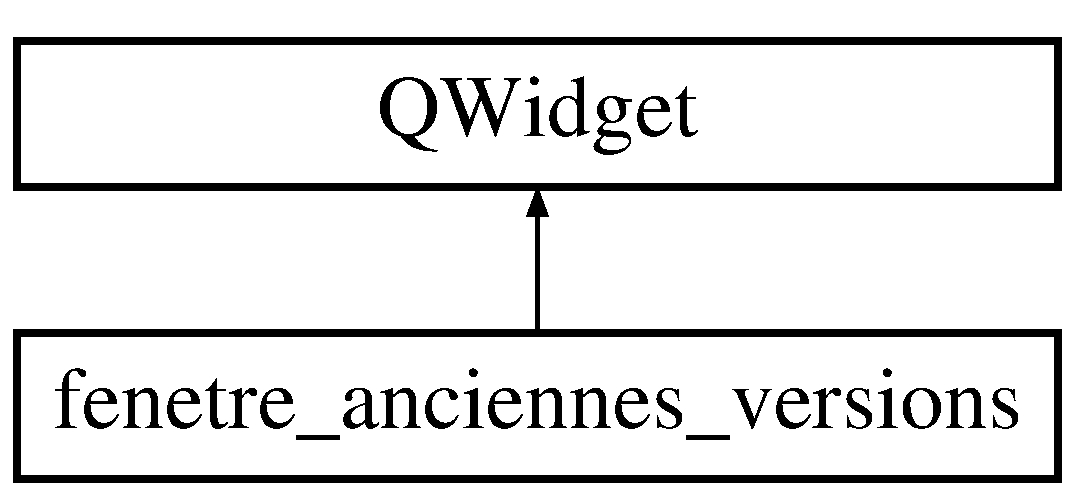
\includegraphics[height=2.000000cm]{classfenetre__anciennes__versions}
\end{center}
\end{figure}
\subsection*{Public Slots}
\begin{DoxyCompactItemize}
\item 
void \hyperlink{classfenetre__anciennes__versions_aff29c8425f322a7e82c950bc77f5ce6d}{choix\+\_\+ancienne\+\_\+version} (Q\+String date)
\begin{DoxyCompactList}\small\item\em Slot appelé lors d\textquotesingle{}un clic sur l\textquotesingle{}une des notes du Q\+List\+Widget. Cela provoque l\textquotesingle{}affichage de la version de la note dans la fenetre principale. \end{DoxyCompactList}\item 
\mbox{\Hypertarget{classfenetre__anciennes__versions_a6a4e824ee33424c6fb8f6fd7331ee900}\label{classfenetre__anciennes__versions_a6a4e824ee33424c6fb8f6fd7331ee900}} 
void \hyperlink{classfenetre__anciennes__versions_a6a4e824ee33424c6fb8f6fd7331ee900}{restaurer} ()
\begin{DoxyCompactList}\small\item\em Slot appelé lors d\textquotesingle{}un clic sur \char`\"{}\+Restaurer\char`\"{}. Supprime la note active et la remplace par la version sélectionnée. \end{DoxyCompactList}\end{DoxyCompactItemize}
\subsection*{Public Member Functions}
\begin{DoxyCompactItemize}
\item 
\hyperlink{classfenetre__anciennes__versions_a4e97516e26d1506c22fade6a4a641c45}{fenetre\+\_\+anciennes\+\_\+versions} (Q\+Widget $\ast$parent)
\begin{DoxyCompactList}\small\item\em Constructeur, initialise la fenetre d\textquotesingle{}affichage des anciennes versions avec un Q\+List\+Widget. \end{DoxyCompactList}\end{DoxyCompactItemize}


\subsection{Detailed Description}
Classe Fenetre d\textquotesingle{}affichage des anciennes versions. 

Cette fenêtre sert à afficher, sélectionner et éventuellement restaurer une version d\textquotesingle{}une note. Les versions sont affichées selon la note depuis laquelle le menu contextuel et l\textquotesingle{}action \char`\"{}\+Anciennces versions\char`\"{} a été activée. 

\subsection{Constructor \& Destructor Documentation}
\mbox{\Hypertarget{classfenetre__anciennes__versions_a4e97516e26d1506c22fade6a4a641c45}\label{classfenetre__anciennes__versions_a4e97516e26d1506c22fade6a4a641c45}} 
\index{fenetre\+\_\+anciennes\+\_\+versions@{fenetre\+\_\+anciennes\+\_\+versions}!fenetre\+\_\+anciennes\+\_\+versions@{fenetre\+\_\+anciennes\+\_\+versions}}
\index{fenetre\+\_\+anciennes\+\_\+versions@{fenetre\+\_\+anciennes\+\_\+versions}!fenetre\+\_\+anciennes\+\_\+versions@{fenetre\+\_\+anciennes\+\_\+versions}}
\subsubsection{\texorpdfstring{fenetre\+\_\+anciennes\+\_\+versions()}{fenetre\_anciennes\_versions()}}
{\footnotesize\ttfamily fenetre\+\_\+anciennes\+\_\+versions\+::fenetre\+\_\+anciennes\+\_\+versions (\begin{DoxyParamCaption}\item[{Q\+Widget $\ast$}]{parent }\end{DoxyParamCaption})}



Constructeur, initialise la fenetre d\textquotesingle{}affichage des anciennes versions avec un Q\+List\+Widget. 


\begin{DoxyParams}{Parameters}
{\em } & Widget/\+Fenetre parente d\textquotesingle{}où provient la fenetre \\
\hline
\end{DoxyParams}


\subsection{Member Function Documentation}
\mbox{\Hypertarget{classfenetre__anciennes__versions_aff29c8425f322a7e82c950bc77f5ce6d}\label{classfenetre__anciennes__versions_aff29c8425f322a7e82c950bc77f5ce6d}} 
\index{fenetre\+\_\+anciennes\+\_\+versions@{fenetre\+\_\+anciennes\+\_\+versions}!choix\+\_\+ancienne\+\_\+version@{choix\+\_\+ancienne\+\_\+version}}
\index{choix\+\_\+ancienne\+\_\+version@{choix\+\_\+ancienne\+\_\+version}!fenetre\+\_\+anciennes\+\_\+versions@{fenetre\+\_\+anciennes\+\_\+versions}}
\subsubsection{\texorpdfstring{choix\+\_\+ancienne\+\_\+version}{choix\_ancienne\_version}}
{\footnotesize\ttfamily void fenetre\+\_\+anciennes\+\_\+versions\+::choix\+\_\+ancienne\+\_\+version (\begin{DoxyParamCaption}\item[{Q\+String}]{date }\end{DoxyParamCaption})\hspace{0.3cm}{\ttfamily [slot]}}



Slot appelé lors d\textquotesingle{}un clic sur l\textquotesingle{}une des notes du Q\+List\+Widget. Cela provoque l\textquotesingle{}affichage de la version de la note dans la fenetre principale. 


\begin{DoxyParams}{Parameters}
{\em date} & \\
\hline
\end{DoxyParams}


The documentation for this class was generated from the following files\+:\begin{DoxyCompactItemize}
\item 
versions.\+h\item 
versions.\+cpp\end{DoxyCompactItemize}

\hypertarget{classfenetre__creation__note}{}\section{fenetre\+\_\+creation\+\_\+note Class Reference}
\label{classfenetre__creation__note}\index{fenetre\+\_\+creation\+\_\+note@{fenetre\+\_\+creation\+\_\+note}}
Inheritance diagram for fenetre\+\_\+creation\+\_\+note\+:\begin{figure}[H]
\begin{center}
\leavevmode
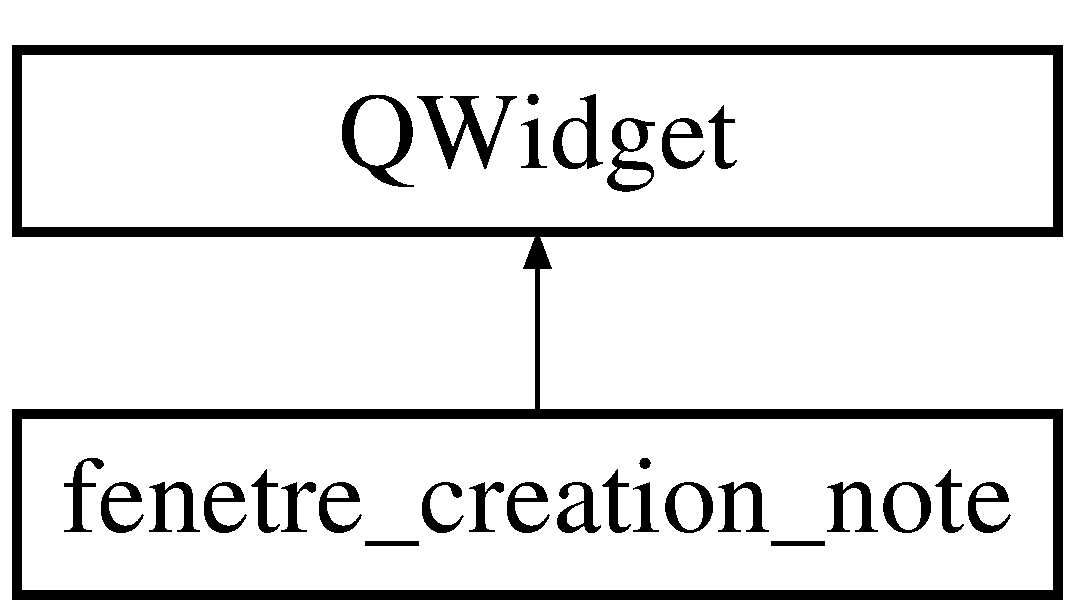
\includegraphics[height=2.000000cm]{classfenetre__creation__note}
\end{center}
\end{figure}
\subsection*{Public Slots}
\begin{DoxyCompactItemize}
\item 
\mbox{\Hypertarget{classfenetre__creation__note_aca59451560c2499954b64ed21db04eb2}\label{classfenetre__creation__note_aca59451560c2499954b64ed21db04eb2}} 
void {\bfseries choisir\+\_\+fichier} ()
\item 
void \hyperlink{classfenetre__creation__note_a148abe3a7d3ba11210f456d4cddce196}{save} ()
\end{DoxyCompactItemize}
\subsection*{Protected Attributes}
\begin{DoxyCompactItemize}
\item 
\mbox{\Hypertarget{classfenetre__creation__note_ae859932afc56d2ba396a4fc5f568f46a}\label{classfenetre__creation__note_ae859932afc56d2ba396a4fc5f568f46a}} 
Q\+V\+Box\+Layout $\ast$ {\bfseries m\+\_\+layout\+\_\+choix}
\item 
\mbox{\Hypertarget{classfenetre__creation__note_a86f29532a57e049e3d45dbe1b4463ad7}\label{classfenetre__creation__note_a86f29532a57e049e3d45dbe1b4463ad7}} 
Q\+Line\+Edit $\ast$ {\bfseries m\+\_\+id}
\item 
\mbox{\Hypertarget{classfenetre__creation__note_aed9003e6b73991a543bee7405b5a3ae7}\label{classfenetre__creation__note_aed9003e6b73991a543bee7405b5a3ae7}} 
Q\+Line\+Edit $\ast$ {\bfseries m\+\_\+titre}
\item 
\mbox{\Hypertarget{classfenetre__creation__note_a7cbded8f75f3efd5680a022149dd0e69}\label{classfenetre__creation__note_a7cbded8f75f3efd5680a022149dd0e69}} 
Q\+Date\+Time {\bfseries m\+\_\+date\+\_\+creat}
\item 
\mbox{\Hypertarget{classfenetre__creation__note_ad0ed47375cd57f9f409c9c764d7d3fa7}\label{classfenetre__creation__note_ad0ed47375cd57f9f409c9c764d7d3fa7}} 
Q\+Date\+Time {\bfseries m\+\_\+date\+\_\+modif}
\item 
\mbox{\Hypertarget{classfenetre__creation__note_aed370c4f6c0aa7639cf30318de49230e}\label{classfenetre__creation__note_aed370c4f6c0aa7639cf30318de49230e}} 
Q\+Label $\ast$ {\bfseries m\+\_\+label\+\_\+date\+\_\+creat}
\item 
\mbox{\Hypertarget{classfenetre__creation__note_a69f335ec51b8cb01185ac131f852bb46}\label{classfenetre__creation__note_a69f335ec51b8cb01185ac131f852bb46}} 
Q\+Label $\ast$ {\bfseries m\+\_\+label\+\_\+date\+\_\+modif}
\item 
\mbox{\Hypertarget{classfenetre__creation__note_a68c7fada71ad687a9d7f1476a900f7f5}\label{classfenetre__creation__note_a68c7fada71ad687a9d7f1476a900f7f5}} 
Q\+Radio\+Button $\ast$ {\bfseries m\+\_\+article}
\item 
\mbox{\Hypertarget{classfenetre__creation__note_a79183b23fc0aea23f53fde89ebf1907e}\label{classfenetre__creation__note_a79183b23fc0aea23f53fde89ebf1907e}} 
Q\+Radio\+Button $\ast$ {\bfseries m\+\_\+tache}
\item 
\mbox{\Hypertarget{classfenetre__creation__note_a449c08c43d3f8d9dccd0a258dbdbace6}\label{classfenetre__creation__note_a449c08c43d3f8d9dccd0a258dbdbace6}} 
Q\+Radio\+Button $\ast$ {\bfseries m\+\_\+media}
\item 
\mbox{\Hypertarget{classfenetre__creation__note_afe742ff20d76a743d300176db81a7b87}\label{classfenetre__creation__note_afe742ff20d76a743d300176db81a7b87}} 
Q\+Text\+Edit $\ast$ {\bfseries m\+\_\+texte}
\item 
\mbox{\Hypertarget{classfenetre__creation__note_a41705de2fed7f8225f33425e711f75df}\label{classfenetre__creation__note_a41705de2fed7f8225f33425e711f75df}} 
Q\+V\+Box\+Layout $\ast$ \hyperlink{classfenetre__creation__note_a41705de2fed7f8225f33425e711f75df}{m\+\_\+layout\+\_\+tache}
\begin{DoxyCompactList}\small\item\em objets qui peuvent être affichés ou non selon la case cochée \end{DoxyCompactList}\item 
\mbox{\Hypertarget{classfenetre__creation__note_ab227c8738d7abaec4971cbfe0906917b}\label{classfenetre__creation__note_ab227c8738d7abaec4971cbfe0906917b}} 
Q\+Spin\+Box $\ast$ {\bfseries m\+\_\+priorite}
\item 
\mbox{\Hypertarget{classfenetre__creation__note_ad436063e4e77a955700f732e431f49f4}\label{classfenetre__creation__note_ad436063e4e77a955700f732e431f49f4}} 
Q\+Combo\+Box $\ast$ {\bfseries m\+\_\+statut}
\item 
\mbox{\Hypertarget{classfenetre__creation__note_a7f9359a4db77422373b0a5183d73a7f2}\label{classfenetre__creation__note_a7f9359a4db77422373b0a5183d73a7f2}} 
Q\+Widget $\ast$ {\bfseries m\+\_\+groupe\+\_\+tache}
\item 
\mbox{\Hypertarget{classfenetre__creation__note_abd8375b439581464e835375fa74102c1}\label{classfenetre__creation__note_abd8375b439581464e835375fa74102c1}} 
Q\+Calendar\+Widget $\ast$ {\bfseries m\+\_\+calendrier}
\item 
\mbox{\Hypertarget{classfenetre__creation__note_ae16a2ce7470e64202a984632d60f233f}\label{classfenetre__creation__note_ae16a2ce7470e64202a984632d60f233f}} 
Q\+Check\+Box $\ast$ {\bfseries m\+\_\+case\+\_\+calendrier}
\item 
\mbox{\Hypertarget{classfenetre__creation__note_acf39fbd867215b30c6f8ae32e2eb4339}\label{classfenetre__creation__note_acf39fbd867215b30c6f8ae32e2eb4339}} 
Q\+Push\+Button $\ast$ {\bfseries m\+\_\+selection\+\_\+fichier}
\item 
\mbox{\Hypertarget{classfenetre__creation__note_ada8843b6be5dd2dff4d99fade6bfada4}\label{classfenetre__creation__note_ada8843b6be5dd2dff4d99fade6bfada4}} 
Q\+String $\ast$ {\bfseries m\+\_\+fichier}
\item 
\mbox{\Hypertarget{classfenetre__creation__note_adfe8b007cfc3075e77c3a1030571cbf5}\label{classfenetre__creation__note_adfe8b007cfc3075e77c3a1030571cbf5}} 
Q\+Push\+Button $\ast$ {\bfseries m\+\_\+save}
\item 
\mbox{\Hypertarget{classfenetre__creation__note_ab3d04eb71646774146d2c12e8f0a53ec}\label{classfenetre__creation__note_ab3d04eb71646774146d2c12e8f0a53ec}} 
Q\+Push\+Button $\ast$ {\bfseries m\+\_\+quit}
\end{DoxyCompactItemize}


\subsection{Member Function Documentation}
\mbox{\Hypertarget{classfenetre__creation__note_a148abe3a7d3ba11210f456d4cddce196}\label{classfenetre__creation__note_a148abe3a7d3ba11210f456d4cddce196}} 
\index{fenetre\+\_\+creation\+\_\+note@{fenetre\+\_\+creation\+\_\+note}!save@{save}}
\index{save@{save}!fenetre\+\_\+creation\+\_\+note@{fenetre\+\_\+creation\+\_\+note}}
\subsubsection{\texorpdfstring{save}{save}}
{\footnotesize\ttfamily void fenetre\+\_\+creation\+\_\+note\+::save (\begin{DoxyParamCaption}{ }\end{DoxyParamCaption})\hspace{0.3cm}{\ttfamily [slot]}}

Si il n\textquotesingle{}y a pas eu d\textquotesingle{}erreur, la note existe déjà

SI la note n\textquotesingle{}existe pas 

The documentation for this class was generated from the following files\+:\begin{DoxyCompactItemize}
\item 
fenetres.\+h\item 
fenetre\+\_\+creation\+\_\+note.\+cpp\end{DoxyCompactItemize}

\hypertarget{classfenetre__creation__relation}{}\section{fenetre\+\_\+creation\+\_\+relation Class Reference}
\label{classfenetre__creation__relation}\index{fenetre\+\_\+creation\+\_\+relation@{fenetre\+\_\+creation\+\_\+relation}}
Inheritance diagram for fenetre\+\_\+creation\+\_\+relation\+:\begin{figure}[H]
\begin{center}
\leavevmode
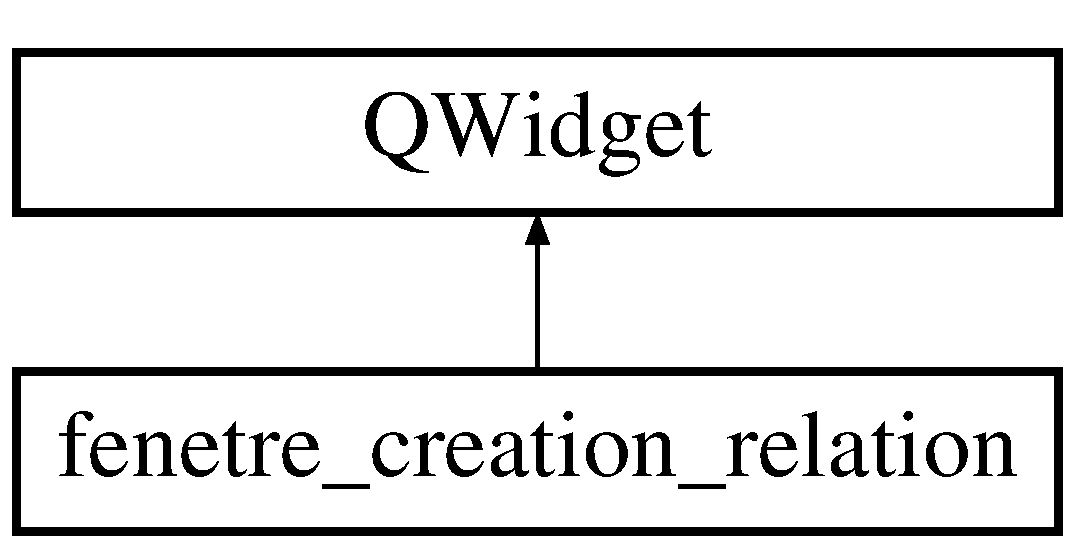
\includegraphics[height=2.000000cm]{classfenetre__creation__relation}
\end{center}
\end{figure}
\subsection*{Public Slots}
\begin{DoxyCompactItemize}
\item 
\mbox{\Hypertarget{classfenetre__creation__relation_ac5b715961f109f3bb403d8ca37faed71}\label{classfenetre__creation__relation_ac5b715961f109f3bb403d8ca37faed71}} 
void {\bfseries affichage\+\_\+couples} ()
\item 
\mbox{\Hypertarget{classfenetre__creation__relation_ad8b233b34d0e2775108683e09a8d966d}\label{classfenetre__creation__relation_ad8b233b34d0e2775108683e09a8d966d}} 
void {\bfseries save\+\_\+couple} ()
\item 
void \hyperlink{classfenetre__creation__relation_af9891e79cff26ef704cfdae9cfa46752}{save\+\_\+relation} ()
\end{DoxyCompactItemize}
\subsection*{Public Member Functions}
\begin{DoxyCompactItemize}
\item 
\mbox{\Hypertarget{classfenetre__creation__relation_ae7f98f1b23dbe45b922b61293348a07f}\label{classfenetre__creation__relation_ae7f98f1b23dbe45b922b61293348a07f}} 
{\bfseries fenetre\+\_\+creation\+\_\+relation} (Q\+Widget $\ast$parent)
\item 
\mbox{\Hypertarget{classfenetre__creation__relation_a843417e0a1f6350f8a3919eb92cf67dd}\label{classfenetre__creation__relation_a843417e0a1f6350f8a3919eb92cf67dd}} 
std\+::vector$<$ \hyperlink{class_couple}{Couple} $\ast$ $>$ {\bfseries get\+Couples} ()
\item 
\mbox{\Hypertarget{classfenetre__creation__relation_a83c62031d4d8d973aca33e38d9079c49}\label{classfenetre__creation__relation_a83c62031d4d8d973aca33e38d9079c49}} 
void {\bfseries lock\+\_\+id\+\_\+relation} (std\+::string titre)
\end{DoxyCompactItemize}


\subsection{Member Function Documentation}
\mbox{\Hypertarget{classfenetre__creation__relation_af9891e79cff26ef704cfdae9cfa46752}\label{classfenetre__creation__relation_af9891e79cff26ef704cfdae9cfa46752}} 
\index{fenetre\+\_\+creation\+\_\+relation@{fenetre\+\_\+creation\+\_\+relation}!save\+\_\+relation@{save\+\_\+relation}}
\index{save\+\_\+relation@{save\+\_\+relation}!fenetre\+\_\+creation\+\_\+relation@{fenetre\+\_\+creation\+\_\+relation}}
\subsubsection{\texorpdfstring{save\+\_\+relation}{save\_relation}}
{\footnotesize\ttfamily void fenetre\+\_\+creation\+\_\+relation\+::save\+\_\+relation (\begin{DoxyParamCaption}{ }\end{DoxyParamCaption})\hspace{0.3cm}{\ttfamily [slot]}}

Si la relation existe déjà 

The documentation for this class was generated from the following files\+:\begin{DoxyCompactItemize}
\item 
fenetres.\+h\item 
fenetre\+\_\+creation\+\_\+relation.\+cpp\end{DoxyCompactItemize}

\hypertarget{class_fen_principale}{}\section{Fen\+Principale Class Reference}
\label{class_fen_principale}\index{Fen\+Principale@{Fen\+Principale}}
Inheritance diagram for Fen\+Principale\+:\begin{figure}[H]
\begin{center}
\leavevmode
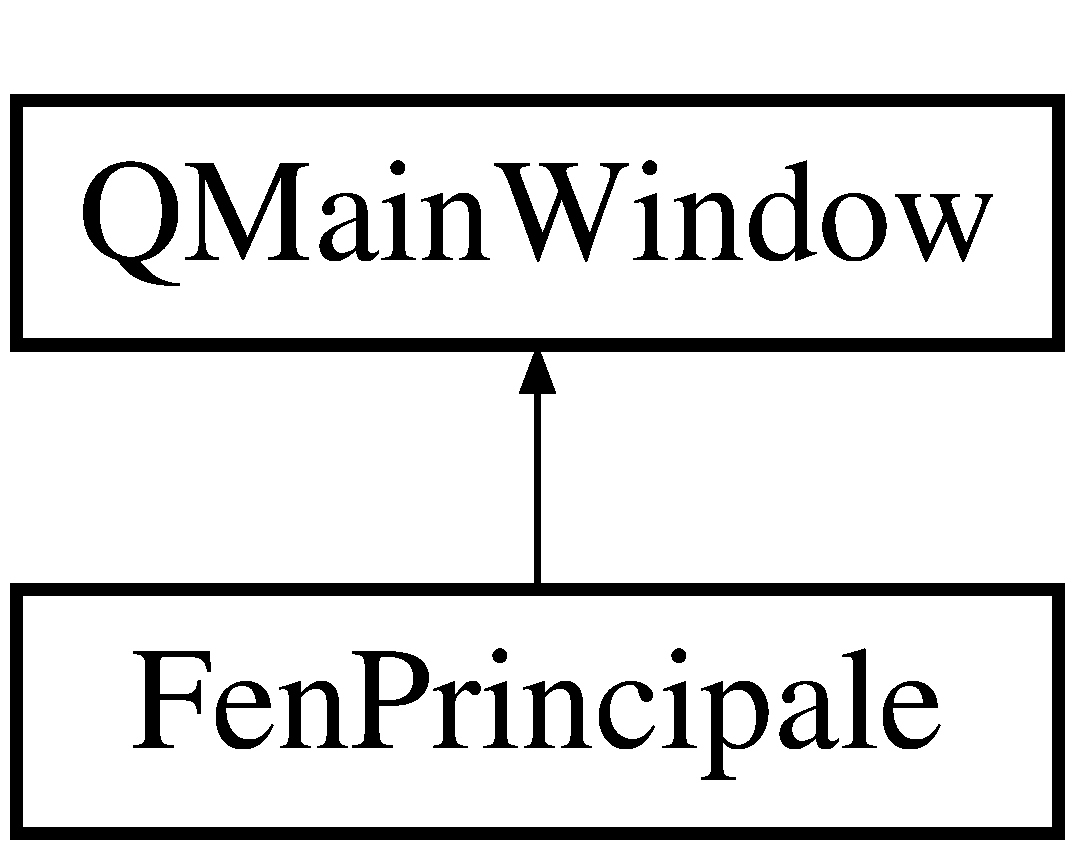
\includegraphics[height=2.000000cm]{class_fen_principale}
\end{center}
\end{figure}
\subsection*{Public Slots}
\begin{DoxyCompactItemize}
\item 
\mbox{\Hypertarget{class_fen_principale_a87ca6c2647ca958c60bac70512da5899}\label{class_fen_principale_a87ca6c2647ca958c60bac70512da5899}} 
void {\bfseries popup} ()
\item 
\mbox{\Hypertarget{class_fen_principale_a59e1d3d260dd7dc4bec7585695dad965}\label{class_fen_principale_a59e1d3d260dd7dc4bec7585695dad965}} 
void {\bfseries popup\+Anciennes\+Versions} ()
\item 
\mbox{\Hypertarget{class_fen_principale_a04c6b879bd8bc7c7ddf164ce9b4273b1}\label{class_fen_principale_a04c6b879bd8bc7c7ddf164ce9b4273b1}} 
void {\bfseries popup\+Creation\+Relation} ()
\item 
\mbox{\Hypertarget{class_fen_principale_a1e99bb2ccb692e8d084b0c667bfd364f}\label{class_fen_principale_a1e99bb2ccb692e8d084b0c667bfd364f}} 
void {\bfseries affichage\+\_\+notes\+\_\+relations} ()
\item 
\mbox{\Hypertarget{class_fen_principale_a6cc4b79a54ed443cced0fb03f7f83619}\label{class_fen_principale_a6cc4b79a54ed443cced0fb03f7f83619}} 
void {\bfseries affichage\+\_\+single\+\_\+note} (Q\+String id, Q\+String date=\char`\"{}\char`\"{})
\item 
\mbox{\Hypertarget{class_fen_principale_a67e142066003277638ed8b7dc67b19e9}\label{class_fen_principale_a67e142066003277638ed8b7dc67b19e9}} 
void {\bfseries affichage\+\_\+single\+\_\+relation} (Q\+String titre)
\item 
\mbox{\Hypertarget{class_fen_principale_a55596abf1539b9b6012fc89f0e9c3d6a}\label{class_fen_principale_a55596abf1539b9b6012fc89f0e9c3d6a}} 
void {\bfseries menu\+Contextuel} (const Q\+Point \&)
\item 
\mbox{\Hypertarget{class_fen_principale_abdbd0250f3c3e037bfa7cd27c5162baf}\label{class_fen_principale_abdbd0250f3c3e037bfa7cd27c5162baf}} 
void {\bfseries supprimer\+Note} ()
\item 
void \hyperlink{class_fen_principale_ab8b916f06d0c149b1411781e7129fab5}{editer\+Note} ()
\item 
\mbox{\Hypertarget{class_fen_principale_a60879a209bf90971f1919a685c9538dd}\label{class_fen_principale_a60879a209bf90971f1919a685c9538dd}} 
void {\bfseries load\+\_\+xml} ()
\item 
\mbox{\Hypertarget{class_fen_principale_adf2a7193704aaf0b73b5b10b3133488c}\label{class_fen_principale_adf2a7193704aaf0b73b5b10b3133488c}} 
void {\bfseries affichage\+\_\+arborescence} (Q\+String id)
\end{DoxyCompactItemize}
\subsection*{Public Member Functions}
\begin{DoxyCompactItemize}
\item 
\hyperlink{class_fen_principale_a529a35ea032da250ad37f7355d1388be}{Fen\+Principale} ()
\item 
\mbox{\Hypertarget{class_fen_principale_a29bdfee5e7a363a205932eeb721dab51}\label{class_fen_principale_a29bdfee5e7a363a205932eeb721dab51}} 
const std\+::string {\bfseries get\+Current\+Note} ()
\end{DoxyCompactItemize}
\subsection*{Protected Member Functions}
\begin{DoxyCompactItemize}
\item 
void \hyperlink{class_fen_principale_ab3ef99b1adb06c0bcc57ea74ca34923e}{creation\+\_\+docks} ()
\item 
\mbox{\Hypertarget{class_fen_principale_aa5ea82e9b0e1c9f93d496cad531ca9e1}\label{class_fen_principale_aa5ea82e9b0e1c9f93d496cad531ca9e1}} 
void {\bfseries creation\+\_\+tabs} ()
\end{DoxyCompactItemize}
\subsection*{Protected Attributes}
\begin{DoxyCompactItemize}
\item 
\mbox{\Hypertarget{class_fen_principale_a3df178449f05185255f1404c09a4b14f}\label{class_fen_principale_a3df178449f05185255f1404c09a4b14f}} 
Q\+Tool\+Bar $\ast$ {\bfseries m\+\_\+toolbar}
\item 
\mbox{\Hypertarget{class_fen_principale_a89d25cfb941913941467b8e4a2d3237b}\label{class_fen_principale_a89d25cfb941913941467b8e4a2d3237b}} 
Q\+V\+Box\+Layout $\ast$ {\bfseries m\+\_\+layout\+\_\+principal}
\item 
\mbox{\Hypertarget{class_fen_principale_a08eeb215ef246ea0b94271054c7834a7}\label{class_fen_principale_a08eeb215ef246ea0b94271054c7834a7}} 
Q\+Dock\+Widget $\ast$ {\bfseries m\+\_\+dock\+\_\+affichage\+\_\+notes}
\item 
\mbox{\Hypertarget{class_fen_principale_a63e6c72aec15e38b352c48c13756863d}\label{class_fen_principale_a63e6c72aec15e38b352c48c13756863d}} 
Q\+List\+Widget $\ast$ {\bfseries m\+\_\+liste\+Notes}
\item 
\mbox{\Hypertarget{class_fen_principale_ad617568d32e9b30f23a764d9e3e5ae06}\label{class_fen_principale_ad617568d32e9b30f23a764d9e3e5ae06}} 
Q\+Dock\+Widget $\ast$ {\bfseries m\+\_\+dock\+\_\+affichage\+\_\+relations}
\item 
\mbox{\Hypertarget{class_fen_principale_a74faa19e906e866482342d4eed32ddb2}\label{class_fen_principale_a74faa19e906e866482342d4eed32ddb2}} 
Q\+List\+Widget $\ast$ {\bfseries m\+\_\+liste\+Relatons}
\item 
\mbox{\Hypertarget{class_fen_principale_adbdeb87d688dfc4845f52f71d31f8d71}\label{class_fen_principale_adbdeb87d688dfc4845f52f71d31f8d71}} 
Q\+Dock\+Widget $\ast$ {\bfseries m\+\_\+dock\+\_\+affichage\+\_\+taches}
\item 
\mbox{\Hypertarget{class_fen_principale_a79ea73002a07dc2a895e1692fa976005}\label{class_fen_principale_a79ea73002a07dc2a895e1692fa976005}} 
Q\+List\+Widget $\ast$ {\bfseries m\+\_\+liste\+\_\+taches}
\item 
\mbox{\Hypertarget{class_fen_principale_abbd84cf259e308941b926573d1bdfe6a}\label{class_fen_principale_abbd84cf259e308941b926573d1bdfe6a}} 
Q\+Widget $\ast$ {\bfseries m\+\_\+fenetre\+\_\+creation}
\item 
\mbox{\Hypertarget{class_fen_principale_a23d1292d5ce03b6375b19daada8ccff9}\label{class_fen_principale_a23d1292d5ce03b6375b19daada8ccff9}} 
\hyperlink{classfenetre__anciennes__versions}{fenetre\+\_\+anciennes\+\_\+versions} $\ast$ {\bfseries m\+\_\+fenetre\+\_\+ancienne\+\_\+versions}
\item 
\mbox{\Hypertarget{class_fen_principale_a5a5ba2e300f3a1da0edbee4fbe629a17}\label{class_fen_principale_a5a5ba2e300f3a1da0edbee4fbe629a17}} 
Q\+Widget $\ast$ {\bfseries m\+\_\+fenetre\+\_\+creation\+\_\+relation}
\item 
\mbox{\Hypertarget{class_fen_principale_a83873dd0fdfb76d95634428393947714}\label{class_fen_principale_a83873dd0fdfb76d95634428393947714}} 
Q\+Tab\+Widget $\ast$ {\bfseries m\+\_\+onglets}
\item 
\mbox{\Hypertarget{class_fen_principale_af48c354467b7971f1da2390d9a656c30}\label{class_fen_principale_af48c354467b7971f1da2390d9a656c30}} 
Q\+Widget $\ast$ {\bfseries m\+\_\+page\+\_\+affichage\+\_\+note}
\item 
\mbox{\Hypertarget{class_fen_principale_a0ce92e619698defb17299db7fac701c5}\label{class_fen_principale_a0ce92e619698defb17299db7fac701c5}} 
Q\+V\+Box\+Layout $\ast$ {\bfseries m\+\_\+layout\+\_\+onglet\+\_\+affichage}
\item 
\mbox{\Hypertarget{class_fen_principale_ad65396826d0d244b45ee0bc34bffb0f2}\label{class_fen_principale_ad65396826d0d244b45ee0bc34bffb0f2}} 
Q\+Label $\ast$ {\bfseries m\+\_\+label\+\_\+\+I\+D\+\_\+note}
\item 
\mbox{\Hypertarget{class_fen_principale_ae3630c82820553ce8aaef41bfd712574}\label{class_fen_principale_ae3630c82820553ce8aaef41bfd712574}} 
Q\+Label $\ast$ {\bfseries m\+\_\+titre\+\_\+note}
\item 
\mbox{\Hypertarget{class_fen_principale_a77b7415d13faa68556a0ebfa8a8272ec}\label{class_fen_principale_a77b7415d13faa68556a0ebfa8a8272ec}} 
Q\+Label $\ast$ {\bfseries m\+\_\+date\+\_\+creation\+\_\+note}
\item 
\mbox{\Hypertarget{class_fen_principale_a4ffed17afb6c84be69fedd43517e03b6}\label{class_fen_principale_a4ffed17afb6c84be69fedd43517e03b6}} 
Q\+Label $\ast$ {\bfseries m\+\_\+date\+\_\+modif\+\_\+note}
\item 
\mbox{\Hypertarget{class_fen_principale_a4b1b4b77ab2700755732450eb6a45a4d}\label{class_fen_principale_a4b1b4b77ab2700755732450eb6a45a4d}} 
Q\+Label $\ast$ {\bfseries m\+\_\+texte\+\_\+note}
\item 
\mbox{\Hypertarget{class_fen_principale_a6f49a22a4798a52a08b4837d218dcf18}\label{class_fen_principale_a6f49a22a4798a52a08b4837d218dcf18}} 
Q\+Label $\ast$ {\bfseries m\+\_\+echeance\+\_\+note}
\item 
\mbox{\Hypertarget{class_fen_principale_ad87eb49d7a0600761d3410453fa7e635}\label{class_fen_principale_ad87eb49d7a0600761d3410453fa7e635}} 
Q\+Label $\ast$ {\bfseries m\+\_\+statut\+\_\+note}
\item 
\mbox{\Hypertarget{class_fen_principale_af4e03cb1d4caa261afe68784ad2ff9b5}\label{class_fen_principale_af4e03cb1d4caa261afe68784ad2ff9b5}} 
Q\+Label $\ast$ {\bfseries m\+\_\+chemin\+\_\+note}
\item 
\mbox{\Hypertarget{class_fen_principale_a03759c7aef2276994e69457a2a4d4ef6}\label{class_fen_principale_a03759c7aef2276994e69457a2a4d4ef6}} 
Q\+Label $\ast$ {\bfseries m\+\_\+priorite\+\_\+note}
\item 
\mbox{\Hypertarget{class_fen_principale_a57b8495c7b3b0aa329648ffb59c723cd}\label{class_fen_principale_a57b8495c7b3b0aa329648ffb59c723cd}} 
Q\+Widget $\ast$ {\bfseries m\+\_\+page\+\_\+affichage\+\_\+relations}
\item 
\mbox{\Hypertarget{class_fen_principale_a1d9603d0f548e700e1ea3ce21f8edb8e}\label{class_fen_principale_a1d9603d0f548e700e1ea3ce21f8edb8e}} 
Q\+Label $\ast$ {\bfseries m\+\_\+titre\+\_\+relation}
\item 
\mbox{\Hypertarget{class_fen_principale_a0a6d9abb0fcea90f1b7d588e086680e5}\label{class_fen_principale_a0a6d9abb0fcea90f1b7d588e086680e5}} 
Q\+Label $\ast$ {\bfseries m\+\_\+description\+\_\+relation}
\item 
\mbox{\Hypertarget{class_fen_principale_afbf019cdafdbf9eb694b944010e8487e}\label{class_fen_principale_afbf019cdafdbf9eb694b944010e8487e}} 
Q\+List\+Widget $\ast$ {\bfseries m\+\_\+liste\+\_\+couples}
\item 
\mbox{\Hypertarget{class_fen_principale_a889991f53d2db1d8f2871d3d1a7a689a}\label{class_fen_principale_a889991f53d2db1d8f2871d3d1a7a689a}} 
Q\+Widget $\ast$ {\bfseries m\+\_\+page\+\_\+arborescence}
\item 
\mbox{\Hypertarget{class_fen_principale_ad9f09d1e423a7d069538c37193f68efc}\label{class_fen_principale_ad9f09d1e423a7d069538c37193f68efc}} 
Q\+V\+Box\+Layout $\ast$ {\bfseries m\+\_\+layout\+\_\+onglet\+\_\+arborescence}
\item 
\mbox{\Hypertarget{class_fen_principale_ab5623b2e095c62d25c37461304cc8de0}\label{class_fen_principale_ab5623b2e095c62d25c37461304cc8de0}} 
Q\+List\+Widget $\ast$ {\bfseries liste\+\_\+ascendants}
\item 
\mbox{\Hypertarget{class_fen_principale_ab1f23c14a220bb4d40b9becfe76435b4}\label{class_fen_principale_ab1f23c14a220bb4d40b9becfe76435b4}} 
Q\+List\+Widget $\ast$ {\bfseries liste\+\_\+descendants}
\item 
\mbox{\Hypertarget{class_fen_principale_a012fbbe56e9e66c7985dc480ba2fa41a}\label{class_fen_principale_a012fbbe56e9e66c7985dc480ba2fa41a}} 
Q\+Label $\ast$ {\bfseries m\+\_\+label\+\_\+arborescence}
\end{DoxyCompactItemize}


\subsection{Constructor \& Destructor Documentation}
\mbox{\Hypertarget{class_fen_principale_a529a35ea032da250ad37f7355d1388be}\label{class_fen_principale_a529a35ea032da250ad37f7355d1388be}} 
\index{Fen\+Principale@{Fen\+Principale}!Fen\+Principale@{Fen\+Principale}}
\index{Fen\+Principale@{Fen\+Principale}!Fen\+Principale@{Fen\+Principale}}
\subsubsection{\texorpdfstring{Fen\+Principale()}{FenPrincipale()}}
{\footnotesize\ttfamily Fen\+Principale\+::\+Fen\+Principale (\begin{DoxyParamCaption}{ }\end{DoxyParamCaption})}

L\+A\+Y\+O\+UT P\+R\+I\+N\+C\+I\+P\+AL 

\subsection{Member Function Documentation}
\mbox{\Hypertarget{class_fen_principale_ab3ef99b1adb06c0bcc57ea74ca34923e}\label{class_fen_principale_ab3ef99b1adb06c0bcc57ea74ca34923e}} 
\index{Fen\+Principale@{Fen\+Principale}!creation\+\_\+docks@{creation\+\_\+docks}}
\index{creation\+\_\+docks@{creation\+\_\+docks}!Fen\+Principale@{Fen\+Principale}}
\subsubsection{\texorpdfstring{creation\+\_\+docks()}{creation\_docks()}}
{\footnotesize\ttfamily void Fen\+Principale\+::creation\+\_\+docks (\begin{DoxyParamCaption}{ }\end{DoxyParamCaption})\hspace{0.3cm}{\ttfamily [protected]}}

2e dock

3e dock \mbox{\Hypertarget{class_fen_principale_ab8b916f06d0c149b1411781e7129fab5}\label{class_fen_principale_ab8b916f06d0c149b1411781e7129fab5}} 
\index{Fen\+Principale@{Fen\+Principale}!editer\+Note@{editer\+Note}}
\index{editer\+Note@{editer\+Note}!Fen\+Principale@{Fen\+Principale}}
\subsubsection{\texorpdfstring{editer\+Note}{editerNote}}
{\footnotesize\ttfamily void Fen\+Principale\+::editer\+Note (\begin{DoxyParamCaption}{ }\end{DoxyParamCaption})\hspace{0.3cm}{\ttfamily [slot]}}

afficher sur le calendrier la date d\textquotesingle{}échéance 

The documentation for this class was generated from the following files\+:\begin{DoxyCompactItemize}
\item 
fenetres.\+h\item 
fenetre\+\_\+principale.\+cpp\item 
versions.\+cpp\end{DoxyCompactItemize}

\hypertarget{struct_notes_manager2_1_1_handler}{}\section{Notes\+Manager2\+:\+:Handler Struct Reference}
\label{struct_notes_manager2_1_1_handler}\index{Notes\+Manager2\+::\+Handler@{Notes\+Manager2\+::\+Handler}}
\subsection*{Public Attributes}
\begin{DoxyCompactItemize}
\item 
\mbox{\Hypertarget{struct_notes_manager2_1_1_handler_a750fdd418013c56b7f49dc2227d41fec}\label{struct_notes_manager2_1_1_handler_a750fdd418013c56b7f49dc2227d41fec}} 
\hyperlink{class_notes_manager2}{Notes\+Manager2} $\ast$ {\bfseries instance}
\end{DoxyCompactItemize}


The documentation for this struct was generated from the following file\+:\begin{DoxyCompactItemize}
\item 
manager.\+h\end{DoxyCompactItemize}

\hypertarget{class_manager}{}\section{Manager$<$ T $>$ Class Template Reference}
\label{class_manager}\index{Manager$<$ T $>$@{Manager$<$ T $>$}}


Classe mère Template abstraite Managers.  




{\ttfamily \#include $<$manager.\+h$>$}

\subsection*{Public Member Functions}
\begin{DoxyCompactItemize}
\item 
void \hyperlink{class_manager_a4eac07f3408be9a9c86273383e282b53}{add} (T \&a\+\_\+ajouter)
\begin{DoxyCompactList}\small\item\em fonction qui vérifie si l\textquotesingle{}id de l\textquotesingle{}objet de type T fourni en paramètre existe déja en parcourant le vector (exeption si c\textquotesingle{}est le cas),et qui l\textquotesingle{}ajoute à l\textquotesingle{}arrièredu vector si ce n\textquotesingle{}est pas le cas. \end{DoxyCompactList}\item 
void \hyperlink{class_manager_a5ad1071a0ca361daea98576c433774c8}{Supprimer} (T \&to\+Delete)
\begin{DoxyCompactList}\small\item\em fonction qui supprime du vector l\textquotesingle{}objet de type T fourni en paramètre \end{DoxyCompactList}\item 
\mbox{\Hypertarget{class_manager_a53786650c42236c2c346cda79cb3cee3}\label{class_manager_a53786650c42236c2c346cda79cb3cee3}} 
const std\+::vector$<$ T $\ast$ $>$ \hyperlink{class_manager_a53786650c42236c2c346cda79cb3cee3}{getobjets} () const
\begin{DoxyCompactList}\small\item\em accesseur en lecture du vector contennat les objets T. \end{DoxyCompactList}\item 
\mbox{\Hypertarget{class_manager_a5f6a3a94521559731ef49005d7669464}\label{class_manager_a5f6a3a94521559731ef49005d7669464}} 
Q\+String \hyperlink{class_manager_a5f6a3a94521559731ef49005d7669464}{get\+Filename} () const
\begin{DoxyCompactList}\small\item\em accesseur en lecture du chemin du fichier xml. \end{DoxyCompactList}\item 
void \hyperlink{class_manager_a5da0f2b938c233c901d1b3f56ce6b77f}{set\+Filename} (const Q\+String \&f)
\begin{DoxyCompactList}\small\item\em met à jour le chemin du du fichier xml. \end{DoxyCompactList}\item 
\mbox{\Hypertarget{class_manager_a18fae41f0e313921265b84b5355ac733}\label{class_manager_a18fae41f0e313921265b84b5355ac733}} 
\hyperlink{class_manager_a18fae41f0e313921265b84b5355ac733}{Manager} ()
\begin{DoxyCompactList}\small\item\em Constructeur de \hyperlink{class_manager}{Manager}, initialise le vector (vide) et definit le chemin par défaut du fichier xml. \end{DoxyCompactList}\item 
\mbox{\Hypertarget{class_manager_aa40cf01ea01fc0fdc029992ff8e8ad74}\label{class_manager_aa40cf01ea01fc0fdc029992ff8e8ad74}} 
virtual \hyperlink{class_manager_aa40cf01ea01fc0fdc029992ff8e8ad74}{$\sim$\+Manager} ()
\begin{DoxyCompactList}\small\item\em destructeur de \hyperlink{class_manager}{Manager} \end{DoxyCompactList}\item 
\mbox{\Hypertarget{class_manager_add6a6361b3ebef4e6e744c2b12f9e57d}\label{class_manager_add6a6361b3ebef4e6e744c2b12f9e57d}} 
virtual void \hyperlink{class_manager_add6a6361b3ebef4e6e744c2b12f9e57d}{load} ()=0
\begin{DoxyCompactList}\small\item\em méthode virtuelle pure pour charger les notes à définir dans les filles \end{DoxyCompactList}\item 
\mbox{\Hypertarget{class_manager_a952734cfd645e6b257ef19ab06d4ded4}\label{class_manager_a952734cfd645e6b257ef19ab06d4ded4}} 
virtual void \hyperlink{class_manager_a952734cfd645e6b257ef19ab06d4ded4}{save} ()=0
\begin{DoxyCompactList}\small\item\em méthode virtuelle pure pour sauvegarder les notes à définir dans les filles \end{DoxyCompactList}\end{DoxyCompactItemize}
\subsection*{Protected Attributes}
\begin{DoxyCompactItemize}
\item 
\mbox{\Hypertarget{class_manager_a1da8f0213719b1f4e7eab848835f77dd}\label{class_manager_a1da8f0213719b1f4e7eab848835f77dd}} 
std\+::vector$<$ T $\ast$ $>$ {\bfseries objets}
\item 
\mbox{\Hypertarget{class_manager_a312ccc5f1d3cf73f9c76b32777f1bcf9}\label{class_manager_a312ccc5f1d3cf73f9c76b32777f1bcf9}} 
Q\+String {\bfseries filename}
\end{DoxyCompactItemize}


\subsection{Detailed Description}
\subsubsection*{template$<$class T$>$\newline
class Manager$<$ T $>$}

Classe mère Template abstraite Managers. 

Cette classe regroupe les attributs et les méthodes communes aux différents Managers. Elle est composée d\textquotesingle{}un vector de template$<$classe T$>$ qui stockera et manipulera les objets T, et d\textquotesingle{}un chemin de fichier (par défaut) qui mène au fichier .xml dans lequel les objets seront sauvegardés. 

\subsection{Member Function Documentation}
\mbox{\Hypertarget{class_manager_a4eac07f3408be9a9c86273383e282b53}\label{class_manager_a4eac07f3408be9a9c86273383e282b53}} 
\index{Manager@{Manager}!add@{add}}
\index{add@{add}!Manager@{Manager}}
\subsubsection{\texorpdfstring{add()}{add()}}
{\footnotesize\ttfamily template$<$class T$>$ \\
void \hyperlink{class_manager}{Manager}$<$ T $>$\+::add (\begin{DoxyParamCaption}\item[{T \&}]{a\+\_\+ajouter }\end{DoxyParamCaption})}



fonction qui vérifie si l\textquotesingle{}id de l\textquotesingle{}objet de type T fourni en paramètre existe déja en parcourant le vector (exeption si c\textquotesingle{}est le cas),et qui l\textquotesingle{}ajoute à l\textquotesingle{}arrièredu vector si ce n\textquotesingle{}est pas le cas. 


\begin{DoxyParams}{Parameters}
{\em T\&} & \+: référence sur l\textquotesingle{}objet à ajouter. \\
\hline
\end{DoxyParams}
\mbox{\Hypertarget{class_manager_a5da0f2b938c233c901d1b3f56ce6b77f}\label{class_manager_a5da0f2b938c233c901d1b3f56ce6b77f}} 
\index{Manager@{Manager}!set\+Filename@{set\+Filename}}
\index{set\+Filename@{set\+Filename}!Manager@{Manager}}
\subsubsection{\texorpdfstring{set\+Filename()}{setFilename()}}
{\footnotesize\ttfamily template$<$class T$>$ \\
void \hyperlink{class_manager}{Manager}$<$ T $>$\+::set\+Filename (\begin{DoxyParamCaption}\item[{const Q\+String \&}]{f }\end{DoxyParamCaption})\hspace{0.3cm}{\ttfamily [inline]}}



met à jour le chemin du du fichier xml. 


\begin{DoxyParams}{Parameters}
{\em filename} & \+: le chemin du nouveau fichier xml. \\
\hline
\end{DoxyParams}
\mbox{\Hypertarget{class_manager_a5ad1071a0ca361daea98576c433774c8}\label{class_manager_a5ad1071a0ca361daea98576c433774c8}} 
\index{Manager@{Manager}!Supprimer@{Supprimer}}
\index{Supprimer@{Supprimer}!Manager@{Manager}}
\subsubsection{\texorpdfstring{Supprimer()}{Supprimer()}}
{\footnotesize\ttfamily template$<$class T$>$ \\
void \hyperlink{class_manager}{Manager}$<$ T $>$\+::Supprimer (\begin{DoxyParamCaption}\item[{T \&}]{to\+Delete }\end{DoxyParamCaption})}



fonction qui supprime du vector l\textquotesingle{}objet de type T fourni en paramètre 


\begin{DoxyParams}{Parameters}
{\em T\&} & \+: référence sur l\textquotesingle{}objet à supprimer. \\
\hline
\end{DoxyParams}


The documentation for this class was generated from the following files\+:\begin{DoxyCompactItemize}
\item 
manager.\+h\item 
manager.\+cpp\end{DoxyCompactItemize}

\hypertarget{classmedia}{}\section{media Class Reference}
\label{classmedia}\index{media@{media}}


Classe fille de note.  




{\ttfamily \#include $<$notes.\+h$>$}

Inheritance diagram for media\+:\begin{figure}[H]
\begin{center}
\leavevmode
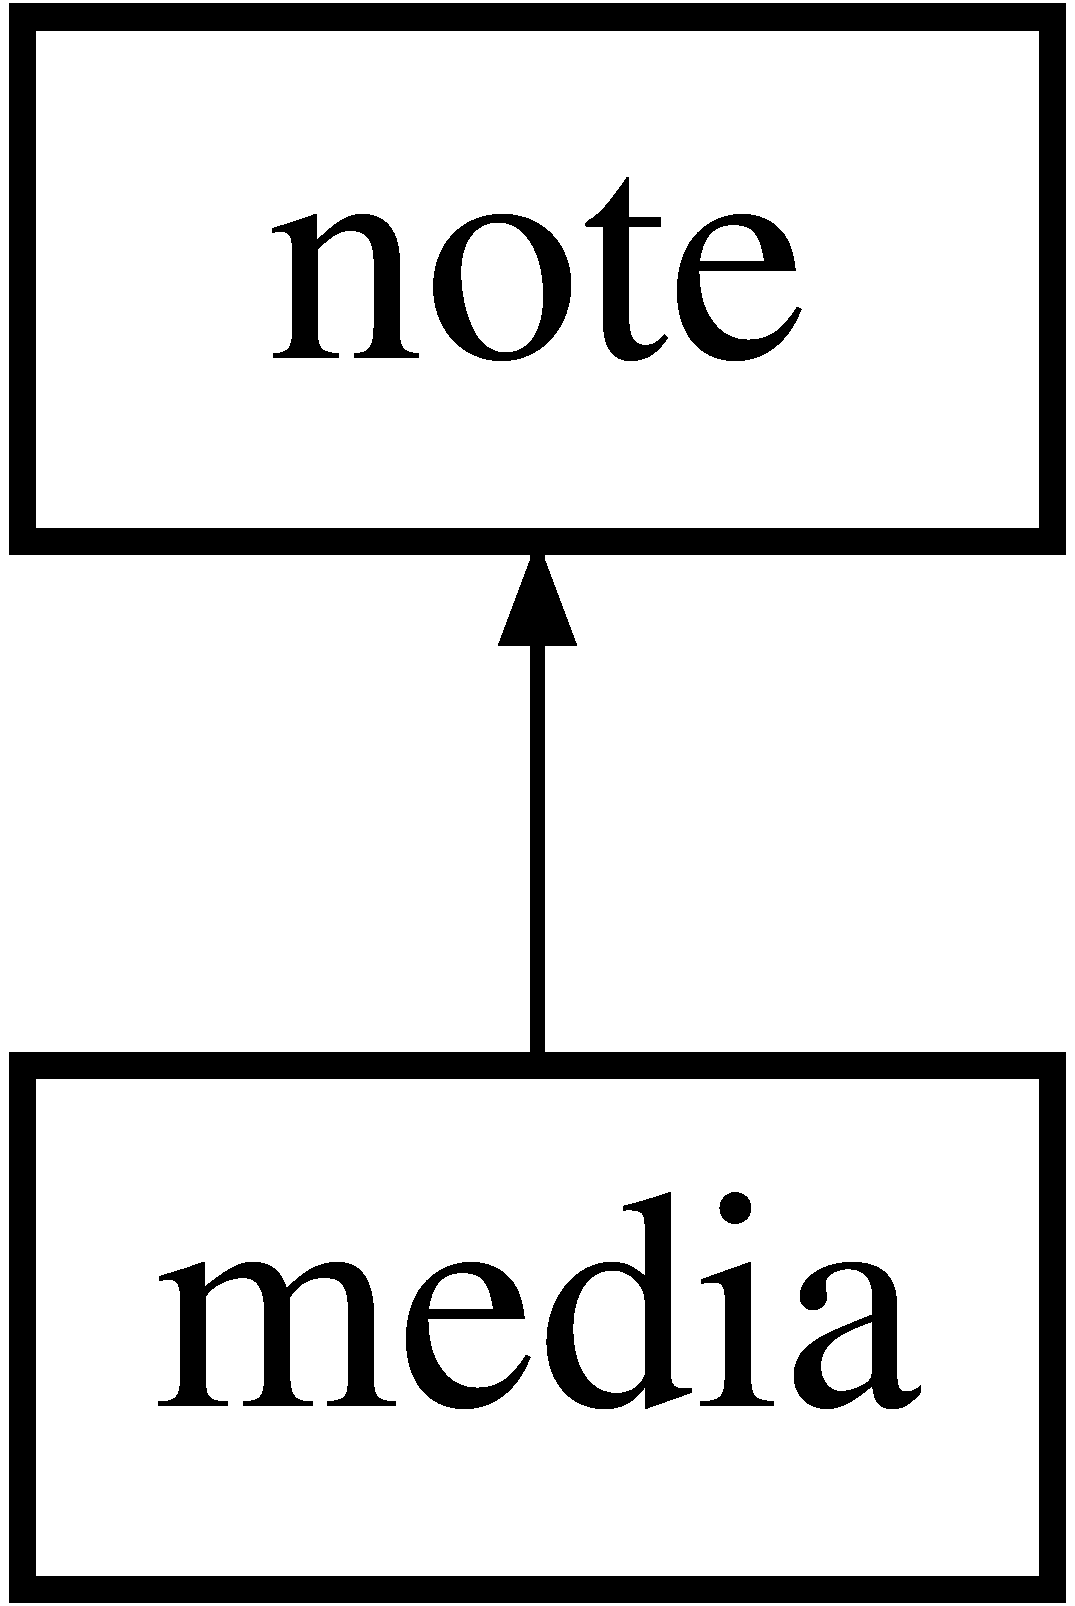
\includegraphics[height=2.000000cm]{classmedia}
\end{center}
\end{figure}
\subsection*{Public Member Functions}
\begin{DoxyCompactItemize}
\item 
\hyperlink{classmedia_a672a7ed2084d2b0d4928dd076bda3919}{media} (const std\+::string i, std\+::string t, std\+::string txt, std\+::string im, std\+::string crea=\char`\"{}\char`\"{}, std\+::string modif=\char`\"{}\char`\"{})
\begin{DoxyCompactList}\small\item\em constructeur utilisant le constructeur de note en ajoutant l\textquotesingle{}attribut correspondant au chemin \end{DoxyCompactList}\item 
\mbox{\Hypertarget{classmedia_a57057824b696efef18a77f814ef086af}\label{classmedia_a57057824b696efef18a77f814ef086af}} 
\hyperlink{classmedia_a57057824b696efef18a77f814ef086af}{media} (const \hyperlink{classmedia}{media} \&media\+\_\+a\+\_\+copier)
\begin{DoxyCompactList}\small\item\em constructeur de recopie \end{DoxyCompactList}\item 
\mbox{\Hypertarget{classmedia_ae9e1c7e0038e5b8036c1f06871ecd19a}\label{classmedia_ae9e1c7e0038e5b8036c1f06871ecd19a}} 
const std\+::string \hyperlink{classmedia_ae9e1c7e0038e5b8036c1f06871ecd19a}{get\+Chemin} () const
\begin{DoxyCompactList}\small\item\em accesseur en lecture du chemin du média \end{DoxyCompactList}\item 
void \hyperlink{classmedia_a9e44b8025a205867c9f853d160da1f6e}{set\+Chemin} (const std\+::string \&text)
\begin{DoxyCompactList}\small\item\em met à jour le chemin du média. \end{DoxyCompactList}\item 
\mbox{\Hypertarget{classmedia_a94e61f8a8d8588dfe947d4a6badd8a93}\label{classmedia_a94e61f8a8d8588dfe947d4a6badd8a93}} 
virtual void \hyperlink{classmedia_a94e61f8a8d8588dfe947d4a6badd8a93}{afficher} (std\+::ostream \&f=std\+::cout) const
\begin{DoxyCompactList}\small\item\em appelle la fonction \hyperlink{classmedia_a94e61f8a8d8588dfe947d4a6badd8a93}{afficher()} de note et affiche le chemin en plus sur la sortie standard. \end{DoxyCompactList}\end{DoxyCompactItemize}
\subsection*{Protected Attributes}
\begin{DoxyCompactItemize}
\item 
\mbox{\Hypertarget{classmedia_a3bd13d97a0f128b7f7d175fd3a006312}\label{classmedia_a3bd13d97a0f128b7f7d175fd3a006312}} 
std\+::string {\bfseries chemin}
\end{DoxyCompactItemize}


\subsection{Detailed Description}
Classe fille de note. 

cette classe est une note possédant un attibut supplémentaire contennant le chemin vers un fichier (texte,image,vidéo...) 

\subsection{Constructor \& Destructor Documentation}
\mbox{\Hypertarget{classmedia_a672a7ed2084d2b0d4928dd076bda3919}\label{classmedia_a672a7ed2084d2b0d4928dd076bda3919}} 
\index{media@{media}!media@{media}}
\index{media@{media}!media@{media}}
\subsubsection{\texorpdfstring{media()}{media()}}
{\footnotesize\ttfamily media\+::media (\begin{DoxyParamCaption}\item[{const std\+::string}]{i,  }\item[{std\+::string}]{t,  }\item[{std\+::string}]{txt,  }\item[{std\+::string}]{im,  }\item[{std\+::string}]{crea = {\ttfamily \char`\"{}\char`\"{}},  }\item[{std\+::string}]{modif = {\ttfamily \char`\"{}\char`\"{}} }\end{DoxyParamCaption})\hspace{0.3cm}{\ttfamily [inline]}}



constructeur utilisant le constructeur de note en ajoutant l\textquotesingle{}attribut correspondant au chemin 


\begin{DoxyParams}{Parameters}
{\em i} & \+: id unique du média \\
\hline
{\em t} & \+: titre du média \\
\hline
{\em txt} & \+: texte décrivant le média \\
\hline
{\em im} & \+: chemin du fichier média \\
\hline
{\em crea} & \+: date de création du média \\
\hline
{\em modif} & \+:date de derniere modification du média \\
\hline
\end{DoxyParams}


\subsection{Member Function Documentation}
\mbox{\Hypertarget{classmedia_a9e44b8025a205867c9f853d160da1f6e}\label{classmedia_a9e44b8025a205867c9f853d160da1f6e}} 
\index{media@{media}!set\+Chemin@{set\+Chemin}}
\index{set\+Chemin@{set\+Chemin}!media@{media}}
\subsubsection{\texorpdfstring{set\+Chemin()}{setChemin()}}
{\footnotesize\ttfamily void media\+::set\+Chemin (\begin{DoxyParamCaption}\item[{const std\+::string \&}]{text }\end{DoxyParamCaption})\hspace{0.3cm}{\ttfamily [inline]}}



met à jour le chemin du média. 


\begin{DoxyParams}{Parameters}
{\em text} & \+: le nouveau chemin. \\
\hline
\end{DoxyParams}


The documentation for this class was generated from the following files\+:\begin{DoxyCompactItemize}
\item 
notes.\+h\item 
notes.\+cpp\end{DoxyCompactItemize}

\hypertarget{classnote}{}\section{note Class Reference}
\label{classnote}\index{note@{note}}


Classe mère abstraite des types de notes.  




{\ttfamily \#include $<$notes.\+h$>$}

Inheritance diagram for note\+:\begin{figure}[H]
\begin{center}
\leavevmode
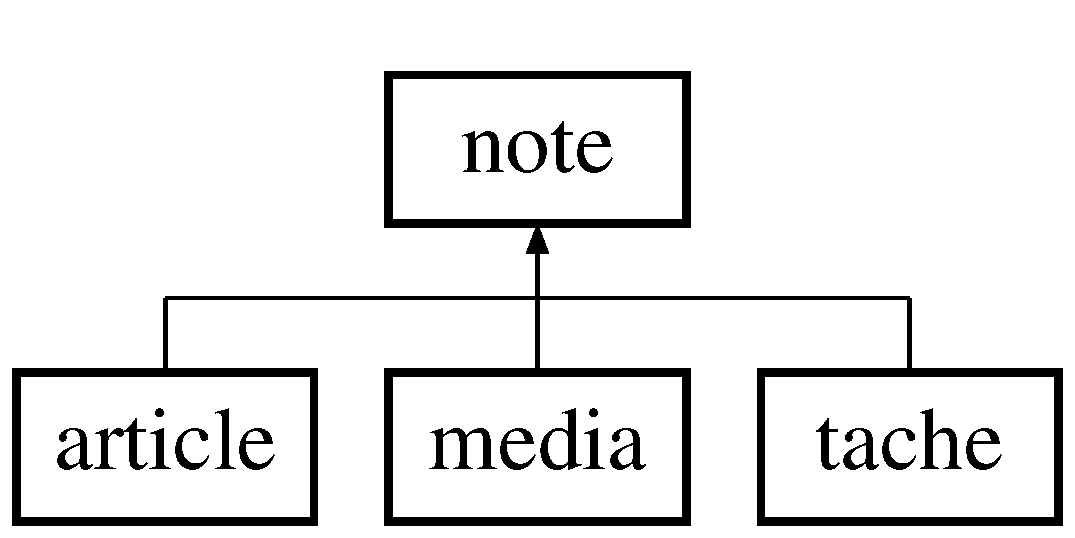
\includegraphics[height=2.000000cm]{classnote}
\end{center}
\end{figure}
\subsection*{Public Member Functions}
\begin{DoxyCompactItemize}
\item 
\hyperlink{classnote_a020b9fbf3603286e010cee5454195302}{note} (std\+::string i, std\+::string t, std\+::string txt, std\+::string crea=\char`\"{}\char`\"{}, std\+::string modif=\char`\"{}\char`\"{})
\begin{DoxyCompactList}\small\item\em Constructeur de notes. \end{DoxyCompactList}\item 
\mbox{\Hypertarget{classnote_a6308957958b5b3b0d82d62d504bbc670}\label{classnote_a6308957958b5b3b0d82d62d504bbc670}} 
const std\+::string \hyperlink{classnote_a6308957958b5b3b0d82d62d504bbc670}{get\+ID} () const
\begin{DoxyCompactList}\small\item\em accesseur en lecture de l\textquotesingle{}id de la note. \end{DoxyCompactList}\item 
\mbox{\Hypertarget{classnote_aa22a099db95d5c357f19838fabe3e5fb}\label{classnote_aa22a099db95d5c357f19838fabe3e5fb}} 
const std\+::string \hyperlink{classnote_aa22a099db95d5c357f19838fabe3e5fb}{get\+Titre} () const
\begin{DoxyCompactList}\small\item\em accesseur en lecture du titre de la note. \end{DoxyCompactList}\item 
\mbox{\Hypertarget{classnote_a5b11e6f329d9b94c80ce7c3bcc2e303f}\label{classnote_a5b11e6f329d9b94c80ce7c3bcc2e303f}} 
const std\+::string \hyperlink{classnote_a5b11e6f329d9b94c80ce7c3bcc2e303f}{get\+Creation} () const
\begin{DoxyCompactList}\small\item\em accesseur en lecture de la date de création de la note. \end{DoxyCompactList}\item 
\mbox{\Hypertarget{classnote_a9ca3911596e876e0747a1ff803a7d930}\label{classnote_a9ca3911596e876e0747a1ff803a7d930}} 
const std\+::string \hyperlink{classnote_a9ca3911596e876e0747a1ff803a7d930}{get\+Modif} () const
\begin{DoxyCompactList}\small\item\em accesseur en lecture de la date de modification de la note. \end{DoxyCompactList}\item 
\mbox{\Hypertarget{classnote_a45af8038b60447374ba961a414910a49}\label{classnote_a45af8038b60447374ba961a414910a49}} 
const std\+::string \hyperlink{classnote_a45af8038b60447374ba961a414910a49}{get\+Texte} () const
\begin{DoxyCompactList}\small\item\em accesseur en lecture du texte de la note. \end{DoxyCompactList}\item 
\mbox{\Hypertarget{classnote_a8cfc267bcce6a99035df33e420a18f38}\label{classnote_a8cfc267bcce6a99035df33e420a18f38}} 
std\+::vector$<$ \hyperlink{classnote}{note} $\ast$ $>$ \& \hyperlink{classnote_a8cfc267bcce6a99035df33e420a18f38}{get\+Old\+Notes} ()
\begin{DoxyCompactList}\small\item\em accesseur du vector contennant les anciennes versions de la note. \end{DoxyCompactList}\item 
void \hyperlink{classnote_a2895efc80041830db954a5af4b0670bf}{set\+Texte} (const std\+::string \&text)
\begin{DoxyCompactList}\small\item\em met à jour le texte de la note. \end{DoxyCompactList}\item 
void \hyperlink{classnote_a70884d3640a6f4440ddb9bd30925b5e7}{set\+Titre} (const std\+::string \&t)
\begin{DoxyCompactList}\small\item\em met à jour le titre de la note. \end{DoxyCompactList}\item 
\mbox{\Hypertarget{classnote_a8fce1df255349a335517128f8e9af543}\label{classnote_a8fce1df255349a335517128f8e9af543}} 
virtual void \hyperlink{classnote_a8fce1df255349a335517128f8e9af543}{afficher} (std\+::ostream \&f=std\+::cout) const
\begin{DoxyCompactList}\small\item\em fonction virtuelle qui affiche les attributs de la note sur la sortie standard. \end{DoxyCompactList}\item 
\mbox{\Hypertarget{classnote_ab90880ae93348a23d0f84f2c2931e0bf}\label{classnote_ab90880ae93348a23d0f84f2c2931e0bf}} 
void \hyperlink{classnote_ab90880ae93348a23d0f84f2c2931e0bf}{set\+Modif} ()
\begin{DoxyCompactList}\small\item\em fonction mettant à jour la date de modificaton avec l\textquotesingle{}heure du système \end{DoxyCompactList}\item 
\mbox{\Hypertarget{classnote_abaece2737aa27cf5efb19e75bedcc41f}\label{classnote_abaece2737aa27cf5efb19e75bedcc41f}} 
virtual \hyperlink{classnote_abaece2737aa27cf5efb19e75bedcc41f}{$\sim$note} ()
\begin{DoxyCompactList}\small\item\em Destructeur de note supprimmant les anciennes versions présentes dans le vector. \end{DoxyCompactList}\end{DoxyCompactItemize}
\subsection*{Protected Attributes}
\begin{DoxyCompactItemize}
\item 
\mbox{\Hypertarget{classnote_a0d600e9189e2de40a0f598be7abf2383}\label{classnote_a0d600e9189e2de40a0f598be7abf2383}} 
std\+::string {\bfseries id}
\item 
\mbox{\Hypertarget{classnote_a5d6bc3a8fea49cec225f3715fe773a39}\label{classnote_a5d6bc3a8fea49cec225f3715fe773a39}} 
std\+::string {\bfseries titre}
\item 
\mbox{\Hypertarget{classnote_ad2368e2d1305df655be46f20dc022871}\label{classnote_ad2368e2d1305df655be46f20dc022871}} 
std\+::string {\bfseries Creation}
\item 
\mbox{\Hypertarget{classnote_a026b48f2e5b88d6cb832f5d23c0b52a7}\label{classnote_a026b48f2e5b88d6cb832f5d23c0b52a7}} 
std\+::string {\bfseries Modif}
\item 
\mbox{\Hypertarget{classnote_a1ae5b932bd6cd2360659548d814628c2}\label{classnote_a1ae5b932bd6cd2360659548d814628c2}} 
std\+::string {\bfseries texte}
\item 
\mbox{\Hypertarget{classnote_add61c3e248f40e52c83c8adb60a81516}\label{classnote_add61c3e248f40e52c83c8adb60a81516}} 
std\+::vector$<$ \hyperlink{classnote}{note} $\ast$ $>$ {\bfseries old\+Notes}
\end{DoxyCompactItemize}


\subsection{Detailed Description}
Classe mère abstraite des types de notes. 

Cette classe regroupe les attributs et les méthodes communes aux différents types de notes, ainsi qu\textquotesingle{}un vector contenant les anciennes versions. Classe à utiliser lors de l\textquotesingle{}implémentatuion d\textquotesingle{}un nouveau type de note. Son but principal est d\textquotesingle{}éviter la redondance de code. 

\subsection{Constructor \& Destructor Documentation}
\mbox{\Hypertarget{classnote_a020b9fbf3603286e010cee5454195302}\label{classnote_a020b9fbf3603286e010cee5454195302}} 
\index{note@{note}!note@{note}}
\index{note@{note}!note@{note}}
\subsubsection{\texorpdfstring{note()}{note()}}
{\footnotesize\ttfamily note\+::note (\begin{DoxyParamCaption}\item[{std\+::string}]{i,  }\item[{std\+::string}]{t,  }\item[{std\+::string}]{txt,  }\item[{std\+::string}]{crea = {\ttfamily \char`\"{}\char`\"{}},  }\item[{std\+::string}]{modif = {\ttfamily \char`\"{}\char`\"{}} }\end{DoxyParamCaption})\hspace{0.3cm}{\ttfamily [inline]}}



Constructeur de notes. 

Ce constructeur crée une nouvelle note avec les paramètres fournis. Si crea (date de création) n\textquotesingle{}est pas renseigné, il s\textquotesingle{}agit d\textquotesingle{}une nouvelle note et le constructeur appelle la fonction format\+Time() qui récupèrela date et l\textquotesingle{}heure du système. cette date est donc affectée à la date de création de la note et aussi à la date de dernière modification. Si ces dattes sont fournis, ils sont affectédd aux attributs correspondants. 
\begin{DoxyParams}{Parameters}
{\em i} & \+: id unique de la note \\
\hline
{\em t} & \+: titre de la note \\
\hline
{\em txt} & \+: texte décrivant la note \\
\hline
{\em creadate} & \+: de création de la note \\
\hline
{\em modif} & \+: date de dernière modification de la note \\
\hline
\end{DoxyParams}


\subsection{Member Function Documentation}
\mbox{\Hypertarget{classnote_a2895efc80041830db954a5af4b0670bf}\label{classnote_a2895efc80041830db954a5af4b0670bf}} 
\index{note@{note}!set\+Texte@{set\+Texte}}
\index{set\+Texte@{set\+Texte}!note@{note}}
\subsubsection{\texorpdfstring{set\+Texte()}{setTexte()}}
{\footnotesize\ttfamily void note\+::set\+Texte (\begin{DoxyParamCaption}\item[{const std\+::string \&}]{text }\end{DoxyParamCaption})\hspace{0.3cm}{\ttfamily [inline]}}



met à jour le texte de la note. 


\begin{DoxyParams}{Parameters}
{\em text} & \+: le nouveau texte de la note. \\
\hline
\end{DoxyParams}
\mbox{\Hypertarget{classnote_a70884d3640a6f4440ddb9bd30925b5e7}\label{classnote_a70884d3640a6f4440ddb9bd30925b5e7}} 
\index{note@{note}!set\+Titre@{set\+Titre}}
\index{set\+Titre@{set\+Titre}!note@{note}}
\subsubsection{\texorpdfstring{set\+Titre()}{setTitre()}}
{\footnotesize\ttfamily void note\+::set\+Titre (\begin{DoxyParamCaption}\item[{const std\+::string \&}]{t }\end{DoxyParamCaption})\hspace{0.3cm}{\ttfamily [inline]}}



met à jour le titre de la note. 


\begin{DoxyParams}{Parameters}
{\em titre} & \+: le nouveau titre de la note. \\
\hline
\end{DoxyParams}


The documentation for this class was generated from the following files\+:\begin{DoxyCompactItemize}
\item 
notes.\+h\item 
notes.\+cpp\end{DoxyCompactItemize}

\hypertarget{class_notes_exception}{}\section{Notes\+Exception Class Reference}
\label{class_notes_exception}\index{Notes\+Exception@{Notes\+Exception}}


Cette classe récupère dans son constructeur un string correspondant à une erreur. On peut catch une erreur de ce type dans les passages sensibles.  




{\ttfamily \#include $<$notes.\+h$>$}

\subsection*{Public Member Functions}
\begin{DoxyCompactItemize}
\item 
\hyperlink{class_notes_exception_a557a49cbc09d8bcbd088ed09edebd086}{Notes\+Exception} (const std\+::string \&message)
\begin{DoxyCompactList}\small\item\em Constructeur. Lors d\textquotesingle{}un test ou d\textquotesingle{}un passage sensible, utiliser un try puis catch un objet de ce type. \end{DoxyCompactList}\item 
std\+::string \hyperlink{class_notes_exception_a5108cf9d122f28f9cb51c0c31c4f2a35}{get\+Info} () const
\begin{DoxyCompactList}\small\item\em Retourne le message d\textquotesingle{}erreur contenu dans l\textquotesingle{}objet de type \hyperlink{class_notes_exception}{Notes\+Exception}. \end{DoxyCompactList}\end{DoxyCompactItemize}


\subsection{Detailed Description}
Cette classe récupère dans son constructeur un string correspondant à une erreur. On peut catch une erreur de ce type dans les passages sensibles. 

\subsection{Constructor \& Destructor Documentation}
\mbox{\Hypertarget{class_notes_exception_a557a49cbc09d8bcbd088ed09edebd086}\label{class_notes_exception_a557a49cbc09d8bcbd088ed09edebd086}} 
\index{Notes\+Exception@{Notes\+Exception}!Notes\+Exception@{Notes\+Exception}}
\index{Notes\+Exception@{Notes\+Exception}!Notes\+Exception@{Notes\+Exception}}
\subsubsection{\texorpdfstring{Notes\+Exception()}{NotesException()}}
{\footnotesize\ttfamily Notes\+Exception\+::\+Notes\+Exception (\begin{DoxyParamCaption}\item[{const std\+::string \&}]{message }\end{DoxyParamCaption})\hspace{0.3cm}{\ttfamily [inline]}}



Constructeur. Lors d\textquotesingle{}un test ou d\textquotesingle{}un passage sensible, utiliser un try puis catch un objet de ce type. 


\begin{DoxyParams}{Parameters}
{\em message} & \+: le message d\textquotesingle{}erreur à afficher \\
\hline
\end{DoxyParams}


\subsection{Member Function Documentation}
\mbox{\Hypertarget{class_notes_exception_a5108cf9d122f28f9cb51c0c31c4f2a35}\label{class_notes_exception_a5108cf9d122f28f9cb51c0c31c4f2a35}} 
\index{Notes\+Exception@{Notes\+Exception}!get\+Info@{get\+Info}}
\index{get\+Info@{get\+Info}!Notes\+Exception@{Notes\+Exception}}
\subsubsection{\texorpdfstring{get\+Info()}{getInfo()}}
{\footnotesize\ttfamily std\+::string Notes\+Exception\+::get\+Info (\begin{DoxyParamCaption}{ }\end{DoxyParamCaption}) const\hspace{0.3cm}{\ttfamily [inline]}}



Retourne le message d\textquotesingle{}erreur contenu dans l\textquotesingle{}objet de type \hyperlink{class_notes_exception}{Notes\+Exception}. 

Navec le essage d\textquotesingle{}erreur en paramètre 
\begin{DoxyParams}{Parameters}
{\em message} & \+: le message d\textquotesingle{}erreur \\
\hline
\end{DoxyParams}
\begin{DoxyReturn}{Returns}
info \+: le message d\textquotesingle{}erreur 
\end{DoxyReturn}


The documentation for this class was generated from the following file\+:\begin{DoxyCompactItemize}
\item 
notes.\+h\end{DoxyCompactItemize}

\hypertarget{class_notes_manager2}{}\section{Notes\+Manager2 Class Reference}
\label{class_notes_manager2}\index{Notes\+Manager2@{Notes\+Manager2}}


Classe fille héritant de \hyperlink{class_manager}{Manager$<$note$>$} et chargée des notes. dispose du Deseign Pattern Singleton.  




{\ttfamily \#include $<$manager.\+h$>$}

Inheritance diagram for Notes\+Manager2\+:\begin{figure}[H]
\begin{center}
\leavevmode
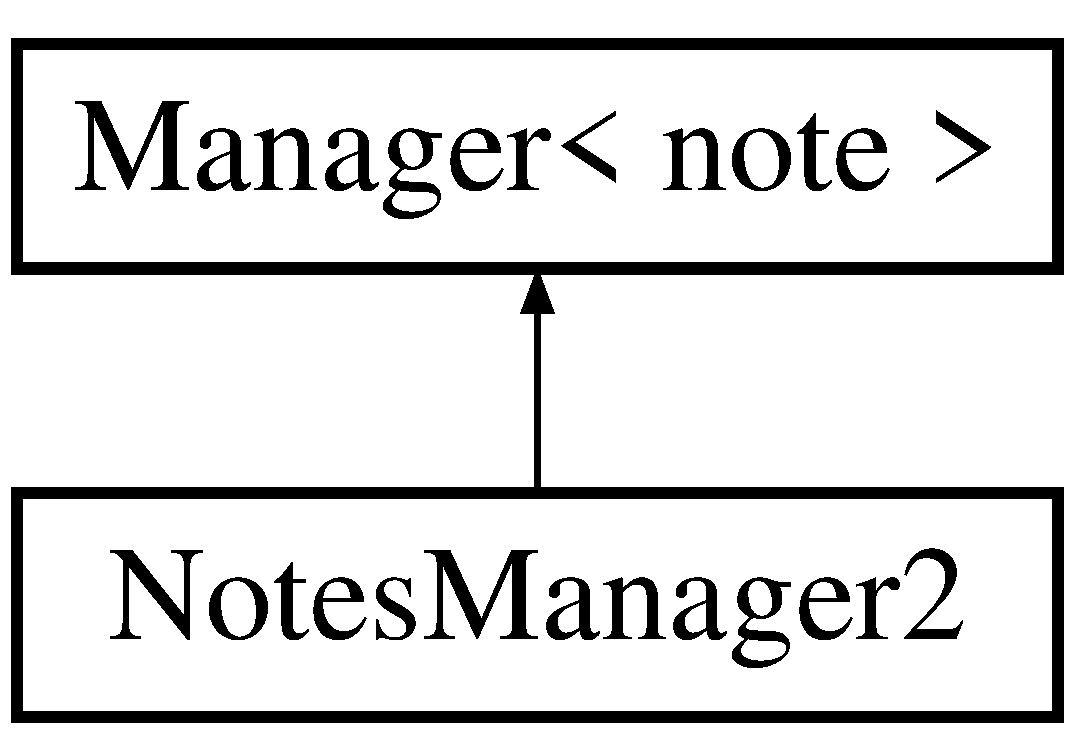
\includegraphics[height=2.000000cm]{class_notes_manager2}
\end{center}
\end{figure}
\subsection*{Public Member Functions}
\begin{DoxyCompactItemize}
\item 
\hyperlink{classnote}{note} \& \hyperlink{class_notes_manager2_a53819d123894c31bbbab66b3d0bf0ff0}{get\+Note} (const std\+::string \&id, const std\+::string \&date=\char`\"{}\char`\"{})
\begin{DoxyCompactList}\small\item\em Méthode retournant une référence sur la note correspondant à l\textquotesingle{}id fourni ou une de ses version antécédente correspondante si une date est fournie. \end{DoxyCompactList}\item 
\mbox{\Hypertarget{class_notes_manager2_ab3812fc5ddfbefa0a03fb2e1f958fd2e}\label{class_notes_manager2_ab3812fc5ddfbefa0a03fb2e1f958fd2e}} 
\hyperlink{classnote}{note} \& {\bfseries get\+Old\+Note} (const std\+::string \&id)
\item 
void \hyperlink{class_notes_manager2_ac020f8488f0f71f92de1e8131a64d943}{Supprimer\+Note} (\hyperlink{classnote}{note} \&to\+Delete, const std\+::string \&date=\char`\"{}\char`\"{})
\begin{DoxyCompactList}\small\item\em Méthode Supprimant une note possédant l\textquotesingle{}id fourni et les couples dans lesquels elle est impliquée. \end{DoxyCompactList}\item 
void \hyperlink{class_notes_manager2_a2248b5b1620b2039fdba9b3c6476c6cc}{load} ()
\begin{DoxyCompactList}\small\item\em Méthode qui charge les données du fichier xml et qui crée les objets qui y sont sauvegardés. \end{DoxyCompactList}\item 
void \hyperlink{class_notes_manager2_a03224a8a150d7d7a40a6633ab2afc7c0}{save} ()
\begin{DoxyCompactList}\small\item\em Méthode chargée de sauvegarder les objets de tous les managers dans le fichier xml. \end{DoxyCompactList}\item 
\mbox{\Hypertarget{class_notes_manager2_a41ec18388f556565d78794ae042511b2}\label{class_notes_manager2_a41ec18388f556565d78794ae042511b2}} 
void \hyperlink{class_notes_manager2_a41ec18388f556565d78794ae042511b2}{check\+References} () const
\begin{DoxyCompactList}\small\item\em Vérifie si les notes contient des références vers d\textquotesingle{}autres notes, et ajoute les couples dans la relation \char`\"{}références\char`\"{}le cas échéant. \end{DoxyCompactList}\end{DoxyCompactItemize}
\subsection*{Static Public Member Functions}
\begin{DoxyCompactItemize}
\item 
\mbox{\Hypertarget{class_notes_manager2_a392bc750d869bacbe50337531213f248}\label{class_notes_manager2_a392bc750d869bacbe50337531213f248}} 
static \hyperlink{class_notes_manager2}{Notes\+Manager2} \& \hyperlink{class_notes_manager2_a392bc750d869bacbe50337531213f248}{get\+Manager} ()
\begin{DoxyCompactList}\small\item\em Renvoie une référence sur le \hyperlink{class_notes_manager2}{Notes\+Manager2} si il existe déja, sinon, le créé.(fait partie du singleton) \end{DoxyCompactList}\item 
\mbox{\Hypertarget{class_notes_manager2_abdc16834a0e2ab7c8b3937674c725a0d}\label{class_notes_manager2_abdc16834a0e2ab7c8b3937674c725a0d}} 
static void \hyperlink{class_notes_manager2_abdc16834a0e2ab7c8b3937674c725a0d}{free\+Manager} ()
\begin{DoxyCompactList}\small\item\em libère l\textquotesingle{}instance unique de \hyperlink{class_notes_manager2}{Notes\+Manager2}.(fait partie du singleton) \end{DoxyCompactList}\end{DoxyCompactItemize}
\subsection*{Additional Inherited Members}


\subsection{Detailed Description}
Classe fille héritant de \hyperlink{class_manager}{Manager$<$note$>$} et chargée des notes. dispose du Deseign Pattern Singleton. 

\subsection{Member Function Documentation}
\mbox{\Hypertarget{class_notes_manager2_a53819d123894c31bbbab66b3d0bf0ff0}\label{class_notes_manager2_a53819d123894c31bbbab66b3d0bf0ff0}} 
\index{Notes\+Manager2@{Notes\+Manager2}!get\+Note@{get\+Note}}
\index{get\+Note@{get\+Note}!Notes\+Manager2@{Notes\+Manager2}}
\subsubsection{\texorpdfstring{get\+Note()}{getNote()}}
{\footnotesize\ttfamily \hyperlink{classnote}{note} \& Notes\+Manager2\+::get\+Note (\begin{DoxyParamCaption}\item[{const std\+::string \&}]{id,  }\item[{const std\+::string \&}]{date = {\ttfamily \char`\"{}\char`\"{}} }\end{DoxyParamCaption})}



Méthode retournant une référence sur la note correspondant à l\textquotesingle{}id fourni ou une de ses version antécédente correspondante si une date est fournie. 


\begin{DoxyParams}{Parameters}
{\em id} & \+: id de la note demmandée \\
\hline
{\em date} & \+: date correspondante à la version recherchée \\
\hline
\end{DoxyParams}
\mbox{\Hypertarget{class_notes_manager2_a2248b5b1620b2039fdba9b3c6476c6cc}\label{class_notes_manager2_a2248b5b1620b2039fdba9b3c6476c6cc}} 
\index{Notes\+Manager2@{Notes\+Manager2}!load@{load}}
\index{load@{load}!Notes\+Manager2@{Notes\+Manager2}}
\subsubsection{\texorpdfstring{load()}{load()}}
{\footnotesize\ttfamily void Notes\+Manager2\+::load (\begin{DoxyParamCaption}{ }\end{DoxyParamCaption})\hspace{0.3cm}{\ttfamily [virtual]}}



Méthode qui charge les données du fichier xml et qui crée les objets qui y sont sauvegardés. 

Appellée au lancement du programme. 

Implements \hyperlink{class_manager_add6a6361b3ebef4e6e744c2b12f9e57d}{Manager$<$ note $>$}.

\mbox{\Hypertarget{class_notes_manager2_a03224a8a150d7d7a40a6633ab2afc7c0}\label{class_notes_manager2_a03224a8a150d7d7a40a6633ab2afc7c0}} 
\index{Notes\+Manager2@{Notes\+Manager2}!save@{save}}
\index{save@{save}!Notes\+Manager2@{Notes\+Manager2}}
\subsubsection{\texorpdfstring{save()}{save()}}
{\footnotesize\ttfamily void Notes\+Manager2\+::save (\begin{DoxyParamCaption}{ }\end{DoxyParamCaption})\hspace{0.3cm}{\ttfamily [virtual]}}



Méthode chargée de sauvegarder les objets de tous les managers dans le fichier xml. 

déclenchée pendant le destructeur, elle appelle les \hyperlink{class_notes_manager2_a392bc750d869bacbe50337531213f248}{get\+Manager()} de chaque \hyperlink{class_manager}{Manager} afin d\textquotesingle{}accéder à leurs vector et sauvegarde leur contennu. Elle définit les balises du xml en fonction de l\textquotesingle{}objet à sauvegarder pour que \hyperlink{class_notes_manager2_a2248b5b1620b2039fdba9b3c6476c6cc}{load()} puisse les reconnaitre. 

Implements \hyperlink{class_manager_a952734cfd645e6b257ef19ab06d4ded4}{Manager$<$ note $>$}.

\mbox{\Hypertarget{class_notes_manager2_ac020f8488f0f71f92de1e8131a64d943}\label{class_notes_manager2_ac020f8488f0f71f92de1e8131a64d943}} 
\index{Notes\+Manager2@{Notes\+Manager2}!Supprimer\+Note@{Supprimer\+Note}}
\index{Supprimer\+Note@{Supprimer\+Note}!Notes\+Manager2@{Notes\+Manager2}}
\subsubsection{\texorpdfstring{Supprimer\+Note()}{SupprimerNote()}}
{\footnotesize\ttfamily void Notes\+Manager2\+::\+Supprimer\+Note (\begin{DoxyParamCaption}\item[{\hyperlink{classnote}{note} \&}]{to\+Delete,  }\item[{const std\+::string \&}]{date = {\ttfamily \char`\"{}\char`\"{}} }\end{DoxyParamCaption})}



Méthode Supprimant une note possédant l\textquotesingle{}id fourni et les couples dans lesquels elle est impliquée. 

Si une date est fournie, on supprime juste la version correspondante sinon, la fonction vérifie parmi les relations si la note est impliquée dans des couples, si c\textquotesingle{}est le cas, les couples sont aussi supprimés. 
\begin{DoxyParams}{Parameters}
{\em id} & \+: id de la note demmandée \\
\hline
{\em date} & \+: date correspondante à la version recherchée \\
\hline
\end{DoxyParams}


The documentation for this class was generated from the following files\+:\begin{DoxyCompactItemize}
\item 
manager.\+h\item 
manager.\+cpp\end{DoxyCompactItemize}

\hypertarget{class_relation}{}\section{Relation Class Reference}
\label{class_relation}\index{Relation@{Relation}}
\subsection*{Public Member Functions}
\begin{DoxyCompactItemize}
\item 
\mbox{\Hypertarget{class_relation_ad80d3956dac01f647bdbb740fdd1cf73}\label{class_relation_ad80d3956dac01f647bdbb740fdd1cf73}} 
{\bfseries Relation} (const std\+::string \&tit, const std\+::string \&desc)
\item 
\mbox{\Hypertarget{class_relation_ad51e21a7258d6980f479dbb21f9e510c}\label{class_relation_ad51e21a7258d6980f479dbb21f9e510c}} 
void {\bfseries add\+Couple} (\hyperlink{class_couple}{Couple} \&couple)
\item 
\mbox{\Hypertarget{class_relation_a5801afed8aa44bde9fd31db7fc019e17}\label{class_relation_a5801afed8aa44bde9fd31db7fc019e17}} 
std\+::vector$<$ \hyperlink{class_couple}{Couple} $\ast$ $>$ \& {\bfseries get\+Couples} ()
\item 
\mbox{\Hypertarget{class_relation_a5cc64235be3be20a82e9ec07486b289c}\label{class_relation_a5cc64235be3be20a82e9ec07486b289c}} 
const std\+::string \& {\bfseries get\+Titre} () const
\item 
\mbox{\Hypertarget{class_relation_a3d43bd45798051dc3aa6015aa225a7c0}\label{class_relation_a3d43bd45798051dc3aa6015aa225a7c0}} 
const std\+::string \& {\bfseries get\+Description} () const
\item 
\mbox{\Hypertarget{class_relation_a481de051dc44065bb816b9b94b5d0c48}\label{class_relation_a481de051dc44065bb816b9b94b5d0c48}} 
void {\bfseries set\+Description} (std\+::string desc)
\end{DoxyCompactItemize}


The documentation for this class was generated from the following file\+:\begin{DoxyCompactItemize}
\item 
relations.\+h\end{DoxyCompactItemize}

\hypertarget{class_relation_manager}{}\section{Relation\+Manager Class Reference}
\label{class_relation_manager}\index{Relation\+Manager@{Relation\+Manager}}


Classe fille héritant de \hyperlink{class_manager}{Manager$<$\+Relation$>$} et chargée des relations. dispose du Deseign Pattern Singleton.  




{\ttfamily \#include $<$manager.\+h$>$}

Inheritance diagram for Relation\+Manager\+:\begin{figure}[H]
\begin{center}
\leavevmode
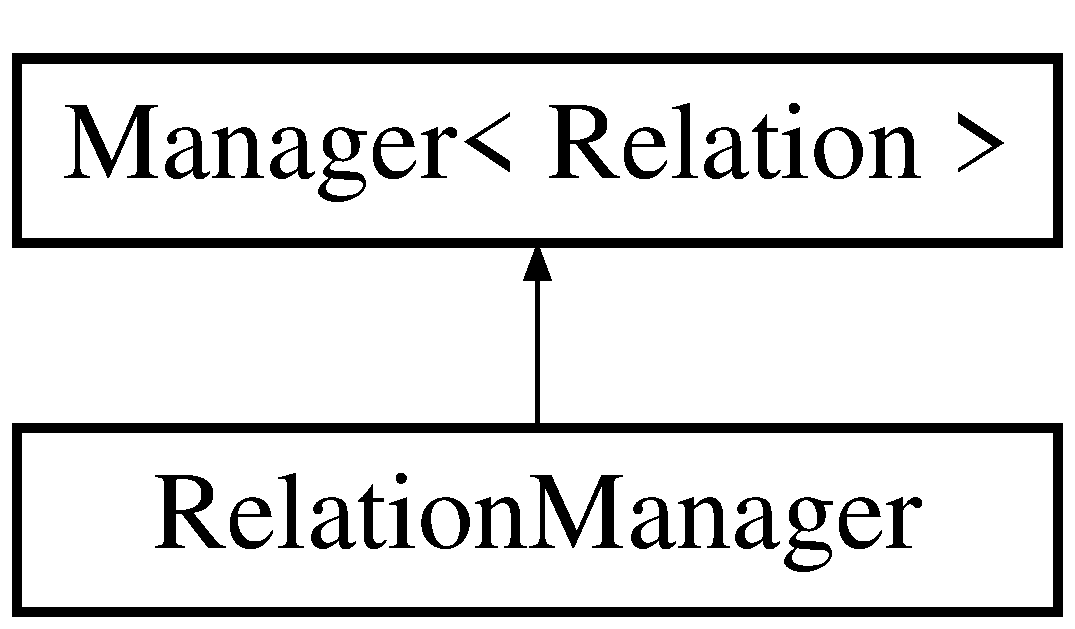
\includegraphics[height=2.000000cm]{class_relation_manager}
\end{center}
\end{figure}
\subsection*{Public Member Functions}
\begin{DoxyCompactItemize}
\item 
\hyperlink{class_relation}{Relation} \& \hyperlink{class_relation_manager_a7e5900e270c2249831355c70b2fd94b8}{get\+Relation} (const std\+::string \&titre)
\begin{DoxyCompactList}\small\item\em Renvoie une référence sur la relation possédant le titre fournit en paramètre. Exeption sinon. \end{DoxyCompactList}\item 
void \hyperlink{class_relation_manager_a2933861a9b973a35031e799ef9d369b5}{add\+Relation} (\hyperlink{class_relation}{Relation} \&relation)
\begin{DoxyCompactList}\small\item\em ajoute une relation au vector du \hyperlink{class_relation_manager}{Relation\+Manager} \end{DoxyCompactList}\item 
\mbox{\Hypertarget{class_relation_manager_a593a538680d22c21a8d1a8dd981f6b44}\label{class_relation_manager_a593a538680d22c21a8d1a8dd981f6b44}} 
void \hyperlink{class_relation_manager_a593a538680d22c21a8d1a8dd981f6b44}{load} ()
\begin{DoxyCompactList}\small\item\em le load général est définit dans \hyperlink{class_notes_manager2}{Notes\+Manager2} \end{DoxyCompactList}\item 
\mbox{\Hypertarget{class_relation_manager_ac9b805487819264d8ef7faab68521822}\label{class_relation_manager_ac9b805487819264d8ef7faab68521822}} 
void \hyperlink{class_relation_manager_ac9b805487819264d8ef7faab68521822}{save} ()
\begin{DoxyCompactList}\small\item\em le save général est définit dans \hyperlink{class_notes_manager2}{Notes\+Manager2} \end{DoxyCompactList}\end{DoxyCompactItemize}
\subsection*{Static Public Member Functions}
\begin{DoxyCompactItemize}
\item 
\mbox{\Hypertarget{class_relation_manager_a525665dcd2599872667dd32f36506f41}\label{class_relation_manager_a525665dcd2599872667dd32f36506f41}} 
static \hyperlink{class_relation_manager}{Relation\+Manager} \& \hyperlink{class_relation_manager_a525665dcd2599872667dd32f36506f41}{get\+Manager} ()
\begin{DoxyCompactList}\small\item\em Renvoie une référence sur le \hyperlink{class_relation_manager}{Relation\+Manager} si il existe déja, sinon, le créé.(fait partie du singleton) \end{DoxyCompactList}\item 
\mbox{\Hypertarget{class_relation_manager_a4c967c4473a2bd29ab558ebf74aed149}\label{class_relation_manager_a4c967c4473a2bd29ab558ebf74aed149}} 
static void \hyperlink{class_relation_manager_a4c967c4473a2bd29ab558ebf74aed149}{free\+Manager} ()
\begin{DoxyCompactList}\small\item\em libère l\textquotesingle{}instance unique de \hyperlink{class_relation_manager}{Relation\+Manager}.(fait partie du singleton) \end{DoxyCompactList}\end{DoxyCompactItemize}
\subsection*{Additional Inherited Members}


\subsection{Detailed Description}
Classe fille héritant de \hyperlink{class_manager}{Manager$<$\+Relation$>$} et chargée des relations. dispose du Deseign Pattern Singleton. 

\subsection{Member Function Documentation}
\mbox{\Hypertarget{class_relation_manager_a2933861a9b973a35031e799ef9d369b5}\label{class_relation_manager_a2933861a9b973a35031e799ef9d369b5}} 
\index{Relation\+Manager@{Relation\+Manager}!add\+Relation@{add\+Relation}}
\index{add\+Relation@{add\+Relation}!Relation\+Manager@{Relation\+Manager}}
\subsubsection{\texorpdfstring{add\+Relation()}{addRelation()}}
{\footnotesize\ttfamily void Relation\+Manager\+::add\+Relation (\begin{DoxyParamCaption}\item[{\hyperlink{class_relation}{Relation} \&}]{relation }\end{DoxyParamCaption})}



ajoute une relation au vector du \hyperlink{class_relation_manager}{Relation\+Manager} 


\begin{DoxyParams}{Parameters}
{\em relation} & \+: référence sur la relation à ajouter. \\
\hline
\end{DoxyParams}
\mbox{\Hypertarget{class_relation_manager_a7e5900e270c2249831355c70b2fd94b8}\label{class_relation_manager_a7e5900e270c2249831355c70b2fd94b8}} 
\index{Relation\+Manager@{Relation\+Manager}!get\+Relation@{get\+Relation}}
\index{get\+Relation@{get\+Relation}!Relation\+Manager@{Relation\+Manager}}
\subsubsection{\texorpdfstring{get\+Relation()}{getRelation()}}
{\footnotesize\ttfamily \hyperlink{class_relation}{Relation} \& Relation\+Manager\+::get\+Relation (\begin{DoxyParamCaption}\item[{const std\+::string \&}]{titre }\end{DoxyParamCaption})}



Renvoie une référence sur la relation possédant le titre fournit en paramètre. Exeption sinon. 


\begin{DoxyParams}{Parameters}
{\em titre} & \+: le titre de la relation à rechercher. \\
\hline
\end{DoxyParams}


The documentation for this class was generated from the following files\+:\begin{DoxyCompactItemize}
\item 
manager.\+h\item 
relations.\+cpp\end{DoxyCompactItemize}

\hypertarget{classtache}{}\section{tache Class Reference}
\label{classtache}\index{tache@{tache}}


Classe fille de note.  




{\ttfamily \#include $<$notes.\+h$>$}

Inheritance diagram for tache\+:\begin{figure}[H]
\begin{center}
\leavevmode
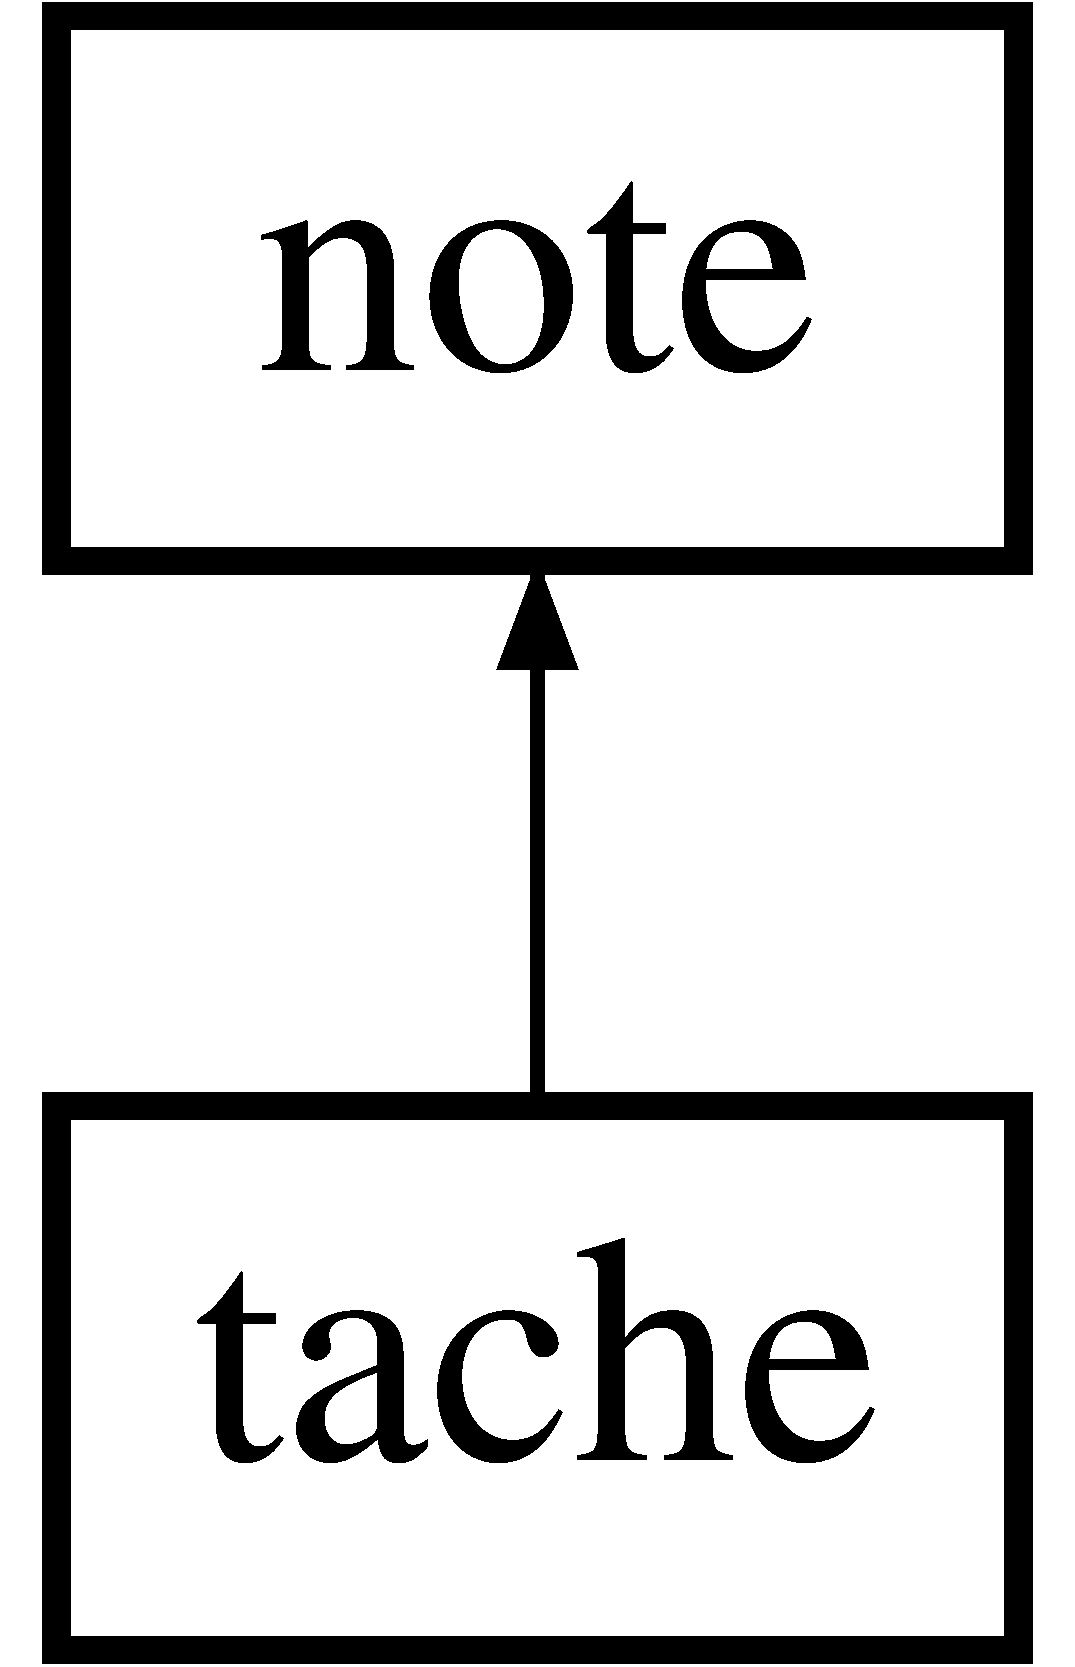
\includegraphics[height=2.000000cm]{classtache}
\end{center}
\end{figure}
\subsection*{Public Member Functions}
\begin{DoxyCompactItemize}
\item 
\hyperlink{classtache_a88ffefc43bb6ee19cb9c6741551ec606}{tache} (const std\+::string i, std\+::string t, std\+::string txt, unsigned int p, std\+::string e, enum etat Status, std\+::string crea=\char`\"{}\char`\"{}, std\+::string modif=\char`\"{}\char`\"{})
\begin{DoxyCompactList}\small\item\em constructeur utilisant le constructeur de note en ajoutant les nouveaux attributs. \end{DoxyCompactList}\item 
\mbox{\Hypertarget{classtache_a6d56536f238c28e385a94ba7db828b00}\label{classtache_a6d56536f238c28e385a94ba7db828b00}} 
\hyperlink{classtache_a6d56536f238c28e385a94ba7db828b00}{tache} (const \hyperlink{classtache}{tache} \&tache\+\_\+a\+\_\+copier)
\begin{DoxyCompactList}\small\item\em constructeur de recopie \end{DoxyCompactList}\item 
\mbox{\Hypertarget{classtache_a6cb88e9c76bba2ba9cdbcb4a24533138}\label{classtache_a6cb88e9c76bba2ba9cdbcb4a24533138}} 
const std\+::string \hyperlink{classtache_a6cb88e9c76bba2ba9cdbcb4a24533138}{getecheance} () const
\begin{DoxyCompactList}\small\item\em accesseur en lecture de l\textquotesingle{}échéance \end{DoxyCompactList}\item 
\mbox{\Hypertarget{classtache_a428f13ec94d058a857a7e060cd69d1f7}\label{classtache_a428f13ec94d058a857a7e060cd69d1f7}} 
enum etat \hyperlink{classtache_a428f13ec94d058a857a7e060cd69d1f7}{get\+Etat} () const
\begin{DoxyCompactList}\small\item\em accesseur en lecture du statut \end{DoxyCompactList}\item 
\mbox{\Hypertarget{classtache_abc6d0d265927c2cd4f7e9cb21643ccbb}\label{classtache_abc6d0d265927c2cd4f7e9cb21643ccbb}} 
unsigned int \hyperlink{classtache_abc6d0d265927c2cd4f7e9cb21643ccbb}{get\+Priorite} () const
\begin{DoxyCompactList}\small\item\em accesseur en lecture de la priorité \end{DoxyCompactList}\item 
void \hyperlink{classtache_a35292bd0bec7a172bf3c70ca3a441153}{set\+Priorite} (int prio)
\begin{DoxyCompactList}\small\item\em met à jour la priorité \end{DoxyCompactList}\item 
void \hyperlink{classtache_adaea7e42b4e6fc8f8903152300968e26}{set\+Echeance} (const std\+::string \&date)
\begin{DoxyCompactList}\small\item\em met à jour l\textquotesingle{}échéance \end{DoxyCompactList}\item 
void \hyperlink{classtache_afd4cda07440e36dc0f47079b110d022e}{set\+Status} (enum etat stat)
\begin{DoxyCompactList}\small\item\em met à jour le statut \end{DoxyCompactList}\item 
\mbox{\Hypertarget{classtache_af319d97c3f228649dce7c24da39307aa}\label{classtache_af319d97c3f228649dce7c24da39307aa}} 
virtual void \hyperlink{classtache_af319d97c3f228649dce7c24da39307aa}{afficher} (std\+::ostream \&f=std\+::cout) const
\begin{DoxyCompactList}\small\item\em appelle la fonction \hyperlink{classtache_af319d97c3f228649dce7c24da39307aa}{afficher()} de note et affiche les attributs de tâche sur la sortie standard. \end{DoxyCompactList}\end{DoxyCompactItemize}
\subsection*{Protected Attributes}
\begin{DoxyCompactItemize}
\item 
\mbox{\Hypertarget{classtache_a50a5f64a76ff14f1467e2b0080618ab9}\label{classtache_a50a5f64a76ff14f1467e2b0080618ab9}} 
unsigned int {\bfseries priorite}
\item 
\mbox{\Hypertarget{classtache_ac49ccbd0d4cd98706d0f45feb4ebe60f}\label{classtache_ac49ccbd0d4cd98706d0f45feb4ebe60f}} 
std\+::string {\bfseries echeance}
\item 
\mbox{\Hypertarget{classtache_acb16537d9ba98cde8d2abc3ac03acf77}\label{classtache_acb16537d9ba98cde8d2abc3ac03acf77}} 
enum etat {\bfseries status}
\end{DoxyCompactItemize}


\subsection{Detailed Description}
Classe fille de note. 

cette classe est une note possédant une priorité sous la forme d\textquotesingle{}un entier, une date d\textquotesingle{}échéance et un statut qui peut etre en\+\_\+attente, en\+\_\+cours ,terminee. 

\subsection{Constructor \& Destructor Documentation}
\mbox{\Hypertarget{classtache_a88ffefc43bb6ee19cb9c6741551ec606}\label{classtache_a88ffefc43bb6ee19cb9c6741551ec606}} 
\index{tache@{tache}!tache@{tache}}
\index{tache@{tache}!tache@{tache}}
\subsubsection{\texorpdfstring{tache()}{tache()}}
{\footnotesize\ttfamily tache\+::tache (\begin{DoxyParamCaption}\item[{const std\+::string}]{i,  }\item[{std\+::string}]{t,  }\item[{std\+::string}]{txt,  }\item[{unsigned int}]{p,  }\item[{std\+::string}]{e,  }\item[{enum etat}]{Status,  }\item[{std\+::string}]{crea = {\ttfamily \char`\"{}\char`\"{}},  }\item[{std\+::string}]{modif = {\ttfamily \char`\"{}\char`\"{}} }\end{DoxyParamCaption})\hspace{0.3cm}{\ttfamily [inline]}}



constructeur utilisant le constructeur de note en ajoutant les nouveaux attributs. 


\begin{DoxyParams}{Parameters}
{\em i} & \+: id unique de la tâche \\
\hline
{\em t} & \+: titre de la tâche \\
\hline
{\em txt} & \+: texte décrivant la tâche \\
\hline
{\em p} & \+: priorité de la tâche \\
\hline
{\em e} & \+: échéance de la tâche \\
\hline
{\em Status} & \+: l\textquotesingle{}état actuel de la tâche \\
\hline
{\em crea} & \+: date de création de la tâche \\
\hline
{\em modif} & \+:date de derniere modification de la tâche \\
\hline
\end{DoxyParams}


\subsection{Member Function Documentation}
\mbox{\Hypertarget{classtache_adaea7e42b4e6fc8f8903152300968e26}\label{classtache_adaea7e42b4e6fc8f8903152300968e26}} 
\index{tache@{tache}!set\+Echeance@{set\+Echeance}}
\index{set\+Echeance@{set\+Echeance}!tache@{tache}}
\subsubsection{\texorpdfstring{set\+Echeance()}{setEcheance()}}
{\footnotesize\ttfamily void tache\+::set\+Echeance (\begin{DoxyParamCaption}\item[{const std\+::string \&}]{date }\end{DoxyParamCaption})\hspace{0.3cm}{\ttfamily [inline]}}



met à jour l\textquotesingle{}échéance 


\begin{DoxyParams}{Parameters}
{\em date} & \+:la nouvelle échéance \\
\hline
\end{DoxyParams}
\mbox{\Hypertarget{classtache_a35292bd0bec7a172bf3c70ca3a441153}\label{classtache_a35292bd0bec7a172bf3c70ca3a441153}} 
\index{tache@{tache}!set\+Priorite@{set\+Priorite}}
\index{set\+Priorite@{set\+Priorite}!tache@{tache}}
\subsubsection{\texorpdfstring{set\+Priorite()}{setPriorite()}}
{\footnotesize\ttfamily void tache\+::set\+Priorite (\begin{DoxyParamCaption}\item[{int}]{prio }\end{DoxyParamCaption})\hspace{0.3cm}{\ttfamily [inline]}}



met à jour la priorité 


\begin{DoxyParams}{Parameters}
{\em prio} & \+:la nouvelle priorité \\
\hline
\end{DoxyParams}
\mbox{\Hypertarget{classtache_afd4cda07440e36dc0f47079b110d022e}\label{classtache_afd4cda07440e36dc0f47079b110d022e}} 
\index{tache@{tache}!set\+Status@{set\+Status}}
\index{set\+Status@{set\+Status}!tache@{tache}}
\subsubsection{\texorpdfstring{set\+Status()}{setStatus()}}
{\footnotesize\ttfamily void tache\+::set\+Status (\begin{DoxyParamCaption}\item[{enum etat}]{stat }\end{DoxyParamCaption})\hspace{0.3cm}{\ttfamily [inline]}}



met à jour le statut 


\begin{DoxyParams}{Parameters}
{\em stat} & \+:le nouveau statut \\
\hline
\end{DoxyParams}


The documentation for this class was generated from the following files\+:\begin{DoxyCompactItemize}
\item 
notes.\+h\item 
notes.\+cpp\end{DoxyCompactItemize}

%--- End generated contents ---

% Index
\backmatter
\newpage
\phantomsection
\clearemptydoublepage
\addcontentsline{toc}{chapter}{Index}
\printindex

\end{document}
